\documentclass[12pt]{article}    % <--- 12pt font
\usepackage[margin=1in]{geometry}% <--- 1 in margin
\linespread{1.5}
\usepackage[utf8]{inputenc}
\usepackage{setspace} 
\usepackage{graphicx}
\usepackage{lscape}
\usepackage{tabularx}
\usepackage{subfigure}
\usepackage{lipsum}
\usepackage{makecell}
\usepackage{tikz}
\usepackage[%  
    colorlinks=true,
    pdfborder={0 0 0},
    linkcolor=blue,
    urlcolor=red,
    linktoc=all,
    citecolor=blue
]{hyperref}
\usepackage{colortbl}
\usepackage[gen]{eurosym}
\usepackage{caption}
\DeclareCaptionLabelFormat{AppendixTables}{A.#2}
\usepackage[title]{appendix}
\usepackage{booktabs}
\graphicspath{ {./images/} }
\usepackage{xcolor}
\newcommand{\MYhref}[3][blue]{\href{#2}{\color{#1}{#3}}}%
\usepackage{pdfpages}
\usepackage[round]{natbib} 
\usepackage[capposition=top]{floatrow}
\usepackage{rotating}
\usepackage[edges]{forest}
\usepackage{blkarray}
\usepackage{dcolumn}
\usepackage{amssymb}
\usepackage{enumitem} 
\usepackage[colorinlistoftodos]{todonotes}
\usepackage{xspace}
\newcommand\nd{\textsuperscript{nd}\xspace}
\newcommand\rd{\textsuperscript{rd}\xspace}
\newcommand\nth{\textsuperscript{th}\xspace} %\th is taken already
\usepackage{array}
\usepackage{blindtext}
\usepackage{times}
\usepackage{mathptmx}
\usepackage{mathtools}
\usepackage{amsmath}
\DeclareUrlCommand\url{\color{blue}}
\newcommand{\underwrite}[3][]{
  \genfrac{}{}{#1}{}{\textstyle #2}{\scriptstyle #3}
}
\usepackage[runin]{abstract}
\setlength{\abstitleskip}{-\parindent} 
\setlength{\absleftindent}{0pt} 
\setlength{\absrightindent}{0pt}
\renewcommand{\abstractnamefont}{\normalfont\bfseries} 
\renewcommand{\abstracttextfont}{\normalfont} 
\abslabeldelim{:\quad} 
\usepackage{adjustbox}
\usepackage{verbatim}




\begin{document}

\title{Bring Together  Belongs Together:\\
The Case of Divided Cities in Europe}
\author{Ketevani Kapanadze}
\date{}  % Optional: Add a specific date
\maketitle

\renewcommand{\thefootnote}{\textdagger} % Change footnote marker to †
\hypersetup{urlcolor=blue} % Ensure hyperlinks are blue
\footnotetext{\textcolor{blue}{\footnotesize \href{ketevani.kapanadze@eruni.org}{ketevani.kapanadze@eruni.org}}, European Research University (ERUNI), Politických vězňů 1419/11 Prague.
\vspace{0.5cm}
\\I am very grateful to Mariola Pytlikova for guidance and encouragement. Thanks to Christian Ochsner, Nikolaus Wolf, Gabriel Alhfeildt, Sebastian Ottinger, Paolo Zacchia, Stepan Mikula, Federico Trionfetti, Lydia Assouad, Christina Felfe, Lukas Makovsky, and Irakli Barbakadze for their constructive comments and suggestions. I also want to extend my gratitude to Christian Lessmann, Felix Roesel, Anna Kremer and all participants in the Regional Economics workshop at the ifo Institute for all valuable discussions. I am very grateful to ANET Lab and KRTK for inviting to the seminar series - I  appreciate all the received feedback, and I would also like to thank Special Thanks to Balazs Lengyel and Zoltan Elekes.  I greatly appreciate all the help I received during the academic job market: from Deborah Novakova and the academic skills center at CERGE-EI. This paper was supported by the Czech Science Foundation (GACR) grant No. 20-31615S and the NPO "Systemic Risk Institute" number LX22NPO5101, funded by European Union - Next Generation EU (Ministry of Education, Youth and , NPO: EXCELES). All remaining errors are mine. }
\renewcommand{\thefootnote}{\arabic{footnote}} % Reset footnote marker to default for the rest of the document



\begin{abstract}
\footnotesize
\par Do spatial concentrations of economic activities have deep historical roots ? This paper explores a unique quasi-natural experiment of opening borders within cities that were historically a single urban entity and were divided due to border shifts following major historical conflicts. After intercity borders were opened, I find that local economic activities, measured by remotely sensed nightlight, became more concentrated close to the pre-division city centers. This raises an important question, what type of border opening is more important in spurring agglomeration, the free movement of goods or of people? When looking into potential mechanisms behind the impact, using national business register databases, I find that proximity to former historical centers is more prominent, particularly after allowance of the free movement of people as a part of the Schengen agreement in 2008, whereas gaining broader market access following the 2004 EU enlargement is less important. I account for two main channels. First, I show that firms in the consumption sectors are more exposed to the free movement of people and are more likely to start operating closer to historical city centers than are firms in the production sectors, which are less affected by local market potentials. Second, I show that cities in which cultural and language differences are not barriers to cross-border cooperation are more influenced by the free movement of than cities where these barriers still exist. Hence, spatial agglomerations near pre-division city centers are more apparent in almost borderless cities.
\par \textbf{Keywords}: Divided cities, borders, historical centre, nightlights, registered firms, Schengen
%\par  \textbf{JEL Codes:}  R12, N14, E65 
\end{abstract}

\newpage

\section{Introduction}
\par The concentration of economic activities within cities has been a subject of interest in urban economics for many years. The concentration of economic activities within cities is a complex phenomenon that can be influenced by a combination of natural factors (first-nature geography) and human interactions (second-nature geography). First-nature geography refers to the inherent characteristics of a location, such as its access to natural resources, climate, topography, and other physical features. These natural advantages can attract economic activities to specific areas. Second-nature geography, on the other hand, focuses on the social and economic interactions that arise from the proximity of firms, people, and infrastructure within urban areas. When businesses and individuals are located close to each other, it can lead to benefits such as knowledge spillovers, reduced transportation costs, labor market efficiencies, and networking opportunities. These agglomeration effects can further enhance the concentration of economic activities in cities. However, distinguishing between the effects of first-nature and second-nature geography can be challenging because they often interact and reinforce each other. For example, a city with favorable natural amenities (first-nature geography) might attract a highly skilled workforce and innovative firms (second-nature geography), leading to a self-reinforcing cycle of economic concentration. Researchers in urban economics strive to disentangle these factors to understand the drivers of economic agglomeration better and to formulate effective urban planning and policy strategies. 

\par This paper aims to address the challenge of finding exogenous variations that are uncorrelated with locational fundamentals by examining a unique quasi-natural setting of removing borders along divided European historical border cities that were once united in the past. I show that local economic activities, measured by remotely sensed nighttime lights (NTL) and by the number of newly established firms, concentrated denser and closer to the pre-division 20th-century centers as Schengen has abolished border barriers and facilitated the free movement of people across Europe. This paper
takes a comprehensive and multinational perspective by examining 22 European historical cities in 10 European countries. It aims to provide a high-resolution analysis by utilizing localized data specific to each historically divided city.
 
\par Divided historical border cities in Europe were one urban unit before the World Wars, and after major international border shifts, cities came apart. For example, the historical German city Frankfurt (Oder) was divided into an East German city - Frankfurt (Oder), and a Polish city - Slubice; the latter was a German suburb called Dammvorstadt until 1945. The lack of cooperation between East Germany and Poland during the communist era created obstacles to cross-border interactions and economic integration. The division of Frankfurt (Oder) and Slubice resulted in economic activities being dispersed away from the pre-division centers due to the restricted movement and limited cooperation between the two separated cities. However, the Eastern enlargement of the European Union in 2004 and Poland's subsequent entry into the Schengen Area in 2008 further facilitated the step-wise development of cross-border cooperation and the free movement of goods, people, and services between the two cities\footnote{It was difficult to freely cross the internal borders between the cities until Poland joined the Schengen Area in  2008.}. After joining Schengen, all border barriers were lifted, enabling divided cities to work together freely once again. I show that economic activities began to re-concentrate toward the pre-division centers. My results suggest that integration policies can bring together what historically belongs together, internal city structures change, and the concentration of economic activities shifts to historical centers. 


\par My paper builds on the large literature on the effect of quasi-natural experiments on the location of economic activity within cities, particularly from a historical perspective. One strand of literature has explored technological inventions in transportation or transportation extensions, e.g.,  \cite{baum2005effects} examines the effects of urban rail transit expansions in sixteen major U.S. cities; \cite{brooks2019vestiges} study the period when streetcars dominated urban transit in Los Angeles county and explore the effects of transportation infrastructure on economic concentration; \cite{heblich2020making} focus on the invention of steam railways in London and analyzes the impacts of transportation innovations on economic clustering. Another strand of literature studies the role of historical policies and historical events within cities, including \cite{arzaghi2008networking}, which investigated the factors influencing the spatial distribution of advertising agencies in Manhattan. They focused on the role of networking externalities and agglomeration economies in shaping the location decisions of advertising agencies; \cite{rossi2010housing} examined the impact of urban revitalization policies on housing externalities in Richmond, Virginia. They focused on concentrated revitalization programs that aimed to improve specific neighborhoods within the city, and \cite{ahlfeldt2015economics} examined the economic consequences of the division and subsequent reunification of Berlin, Germany. It seems as if there is some consensus on understanding the sources and dynamics of economic concentration within the cities. However, the area is still under-researched. The existing literature often focuses on specific cities, which may limit the generalizability of the findings. Each city has its unique characteristics, historical background, and economic structure, which can lead to different channels of agglomeration forces at play. 


\par This paper contributes to the stream of literature by exploring a unique quasi-natural experiment of opening borders within cities, which used to be  one city in the past and were divided following major historical conflicts. The closest to my work is a study by \cite{ahlfeldt2015economics}, where authors study how the reunification of Berlin affected the city’s economic landscape, including
the role of historical city centers and their transformation in the post-reunification era.
My central contribution is assessing border effects for a different type of border (e.g., with its different historical and institutional circumstances) than the imposition and removal of the Iron Curtain. In contrast to their study, my paper which studies cities that were split into two different countries with different languages and cultures, allows me to shed some light on different mechanisms and channels. 


\par My paper's setting of multiple border cities and detailed NTL and business register data allows me to study different underlying economic mechanisms  and channels of agglomeration forces, something that has not been studied yet, to the best of my knowledge. The paper has the main findings in the following three aspects. 


\par First, the implementation of the free movement of people policy in 2008 had a significant impact on reorienting economic and human activities towards pre-division city centers. However, the "borderless market" or free movement of goods, services, and capital in 2004 did not have the same effect. This indicates that factors other than the movement of goods and capital, such as the direct engagement and interaction of people, play a more significant role in driving economic concentration near historical centers.


\par Second, city heterogeneity allowed me to investigate the role of language and cultural closeness between divided city pairs. While historical centers tend to be hubs of social activities, language similarity should enhance participation and integration into cross-national networks.  Therefore, I show that businesses are more likely to concentrate on areas where they can effectively communicate and engage with the local and foreign markets. I show that economic activities concentrate closer to former historical centers in city pairs where lexical similarities are high between languages in divided cities and cultural and language differences are not barriers to cross-border cooperation. 


\par Third, using a data set on registered firms in divided border cities, I show that the consumption-oriented sectors concentrate near pre-division centers.  Firms in the consumption sector facilitate greater interaction and connectivity among local and foreign people. I show that  restaurants, cafes, and cultural and entertainment venues started operating in a close radius of former historical centers after removing all types of borders in divided cities. Customers from both sides of the formerly united city can come to these areas, leading to increased physical movement and social interactions. This increased human mobility could create shared spaces, fostering a sense of togetherness and community within the divided city.

\par This paper also contributes to the European integration literature. While there has been researched on the broader impacts of EU integration on regional development and urbanization patterns \textit{across} European cities (\citealp{Brakman2012}; 
\citealp{brulhart2018trade}; 
\citealp{Heider2019}), the concentration and spatial distribution of economic activities \textit{inside} cities in the course of European integration have not been studied before. 

\par The rest of the paper is organized as follows: Section 2 introduces the history of the study area with a particular focus on city division and historical city centers; Section 3 explains the data; Section 4 presents the empirical framework and main results; Section 5 discuss the channels; Section 6 concludes the paper.

\subsection{Historty of Study Area}

\subsubsection{City Division}
\par The geographical division of some European cities occurred mainly after two major shocks, World Wars  I and II. WWI brought about the collapse of multinational empires - the Russian, Ottoman, Austro-Hungarian, and German. Consequently, new borderlines were drawn in Europe, and some European cities were divided into separated city parts due to conflicts and border shifts. Cities that were united at the beginning of the 20th century and later divided are located along the borders of Austria-Slovenia, Hungary-Slovakia, Poland-Czechia, Austria-Czechia, and Latvia-Estonia. These city locations are illustrated in \hyperlink{Figure 2.1}{Figure 2.1}, and a detailed description is provided in \hyperlink{Table 2.1}{Table 2.1}.




\begin{figure}[H] \hypertarget{Figure 2.1}{}
\renewcommand\thefigure{2.1} 
\RawCaption{\caption{Divided Border Cities in Europe} }\vskip\captionskip
\floatbox[{\captop}]{figure}[\FBwidth]
    {}
   {
    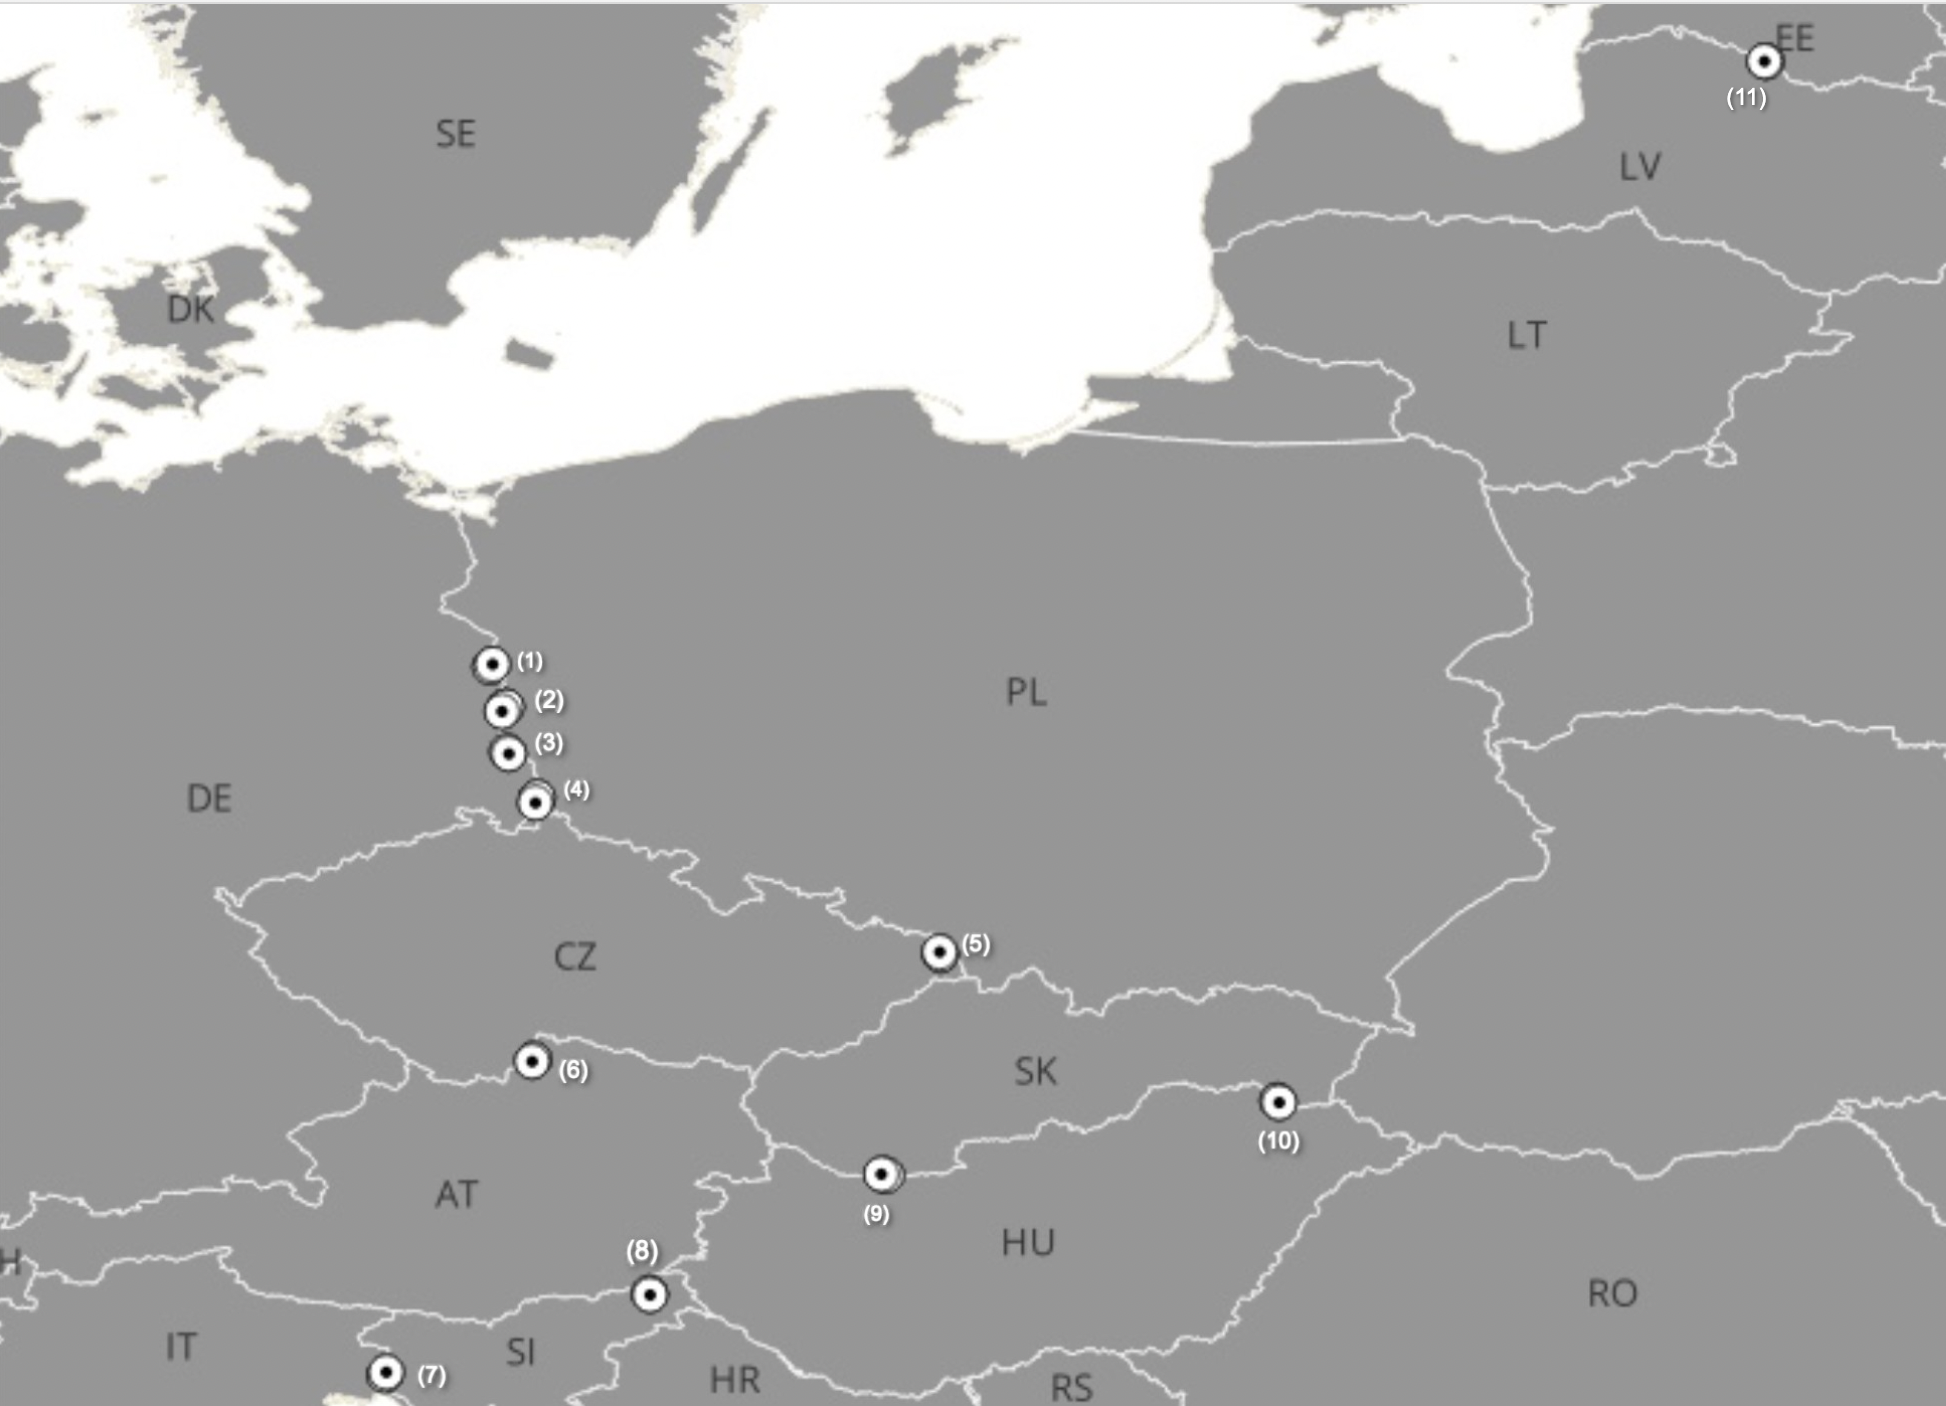
\includegraphics[scale=0.45]{photos/dividedcities}
    \floatfoot{ 
\scriptsize 
\textit{Source:} Author's elaboration based on GISCO shapefiles. \\\textit{Notes}: Circles on the map illustrate 22 divided cities in 10 European countries, i.e., Germany (DE), Poland (PL), Czechia (CZ), Slovenia (SI), Slovakia (SK), Austria (AT), Hungary (HU), Italy (IT), Estonia (EE), and Latvia (LV). Divided cities  are (1) Frankfurt (Oder) - Slubice, (2) Zgorzelec - Gorlitz, (3) Guben - Gubin, (4) Leknica - Bad Muskau, (5) Ceske Teshin - Cieszyn, (6) Gmund - Ceske Velenice, (7) Nova Gorica - Gorizia, (8) Bad Radkersburg - Gornja Radgona, (9) Komarom - Komarno, (10) Satoraljaujhely - Slovenske Nové Mesto, (11) Valga - Valka}}
\end{figure}


\par  After World War I (1914-1918), there were significant territorial adjustments and the creation of a new nation. After years of conflict between countries, in total, 12 historical border cities were divided. As for World War II (1939-1945), there were also significant territorial changes and political shifts. Therefore, ten historical border cities were divided due to this tension. 

\par During the first half of the 20th century, other newly founded republics of Estonia and Latvia entered into a conflict over the historical city of Walk. In 1919, the city was divided; the Estonian part was called Valga, and the Latvian side, Valka. The Baltic states were invaded and occupied from June 1940 until 1990 by the Soviet Union\footnote{The historical city of Walk was \textit{united} in the Soviet Union.}. In 1991, Latvia and Estonia declared independence. 


\par After WWI, the newly created independent states of Poland and Czechoslovakia engaged in conflict over the area of the city of Teschen. Because the highest authorities in both nations could not reach a consensus, the city of Teschen was divided into a Polish part, Cieszyn, and the Czechoslovak area became Cesky Tesin in 1919. Further, until 1918, Ceske Velenice was part of the Austrian city of Gmund. At the end of WWI, following the Treaty of Saint-Germain-en-Laye (1919), the territory officially became part  of Czechoslovakia  - a new Czech city. Similarly, Gornja Radgona, which is located on the northern edge of Slovenia, was historically a part of the Austrian city of Bad Radkersburg - a divided city on the other side of the Mura River. They were divided in 1919 when the state of Styria was divided into Austria and Slovenia. Further, in the same period, the city of Komárom was divided along the national border between Hungary and Czechoslovakia (today, Slovakia), creating the city of Komarno in Slovakia and Komarom in Hungary. 

\begin{table}[H]\hypertarget{Table 2.1}{}
\renewcommand\thetable{2.1}
\centering
\scriptsize
\RawCaption{\caption{Divided Cities in Europe}}
\vskip\captionskip
\floatbox[{\captop}]{figure}[\FBwidth]
    {}
{
\def\sym#1{\ifmmode^{#1}\else\(^{#1}\)\fi}
\noindent\makebox[\linewidth]{
\begin{tabular}{|l|l|l|l|l|l|}
\hline 
\textbf{Historical City} & \textbf{Divided City (A)}& \textbf{Divided City (B) }              &\textbf{Rise of Borders}  & \textbf{Fall of Borders }  & \textbf{ 20th century centers}\\                                          
\hline
\hline
Frankfurt  & Frankfurt (Oder) (DE)                                           & 
  Slubice (PL) & 1945                   
                  &  {2008}          &  Museum Viadrina (DE)\\
                  \hline
                Gorlitz                  & Gorlitz (DE)                                                     & Zgorzelec (PL)
                & 1945 & {2008}        & Historical \& Cultural Museum (DE) \\
\hline
Guben                    & Guben (DE)                                                       & Gubin (PL)         &1945                             &  {2008}          & City \& Industry Museum (DE)\\
\hline
Bad Muskau*               & Bad Muskau (DE)                                                 & Leknica (PL)  & 1945                &  {2008}          & Schlobvorwerk (DE) \\ 
\hline
 Gorizia                  & Gorizia (IT)                                                      & Nova Goricia (SI)    
 
 & 1945  & {2008}          & Palazzo Lantieri (IT)\\
\hline
 Bad Radkersburg*          & Bad Radkersburg (AT)                                            & 
  Gornja
  Radgona (SI)
       &  1919                 & {2008}      & Frauenkirche Bad Radkersburg (DE)\\
\hline
Komarom                  & Komarom (HU)                                                    & Komarno (SK)                      & 1919                 &   {2008}          & Gyorgy Klapka Museum (HU) \\
 \hline
 Satoraljaujhely*          & Satoraljaujhely (HU)                                            & 
  Slovenske
  Nove Mesto (SK)
   & 1919               & {2008}          &  Kazinczy Ferenc Muzeum (HU)\\
\hline
 Teschen                  & Cieszyn (PL)                                                     & Cesky Tesin (CZ)               & 1919                  & {2008}          & Museum of Cieszyn Silesia (PL)\\

         \hline
Gmund                    & Gmund (AT)                                                      & Ceske Velenice (CZ)                & 1919             &  {2008}          & Schloss (Castle) Gmund (AT)\\
 
   \hline
 Walk                     & Valka (LV)                                                       & Valga (EE)                         & 1919             & {2008}        & Valga Museum (EE)
 \\
\hline
 \end{tabular} 

 }
    \floatfoot{\scriptsize \textit{Source:} Author's elaboration.}
    }
\end{table}
%  \justifying \scriptsize\textit{Notes}: The first column shows the names of historical cities. The second and third columns present the names of cities after they were divided. The fourth column shows the year a city was divided and intra-city borders were established. The fifth column indicates when border controls were lifted. The sixth column displays the names of all historical centers - historical museums, plazas, churches, and city halls. I dropped some divided European cities from the sample due to their small sizes, including Laufenburg (Laufenburg, Germany and Laufenburg, Switzerland) and Rheinfelden (Rheinfelden, Germany and Rheinfelden, Switzerland). During the Soviet era, Valga and Valka were once united and then separated again in 1992 when the Soviet Union was dissolved. Cities denoted by an asterisk (*) are not part of the sample due to their small size.




\par At the end of World War II, Europe underwent further significant changes to  the locations of its internal international borders. For example, in 1945, after the defeat of Nazi Germany, the Oder–Neisse line became Poland’s western and Germany’s Eastern border. At the end of WWII, a new international border was established between Germany and Poland, dividing four historical border cities. Thus, four new border city pairs emerged along the new borderline, including Frankfurt (Oder)-Slubice, Gubin-Guben, Gorlitz-Zgorlec, and Bad Muskau-Leknica. 


\par In 1947, after WWII, Italy signed a peace treaty with Yugoslavia (today, Slovenia) and handed over half of Gorizia\footnote{Gorizia and Nova Gorica were often compared to West and East Berlin before and after Iron Curtain.}. A new city, Nova Gorica, was built on the other side of the Slovenian border area, and the rest of the city of Gorizia remained in Italy. When Yugoslavia broke up in 1992, the physical border remained between the two cities, forming the dividing line between Italy and Slovenia. 

\par These barriers lasted decades until New Member States (Czechia, Slovakia, Poland, Hungary, Slovenia, Latvia, Estonia) started stepwise lifting borders in 2004. Though the physical barriers still remained. The final step of pulling together the divided cities was in early 2008 after countries signed the Schengen Agreement\footnote{See \hyperlink{Figure 2.C.1}{Figure 2.C.1}, for photo example illustration.}. Therefore, the historical cities physically returned to their pre-division conditions.


\subsubsection{Historical City Centers (HCTRs)}

\par The information regarding the historical cities' 20th century centers listed in \hyperlink{Table 2.1}{Table 2.1} before their division is based on a combination of general historical knowledge and the identification of the oldest buildings in each city. 

\par In divided border cities, the historical significance and symbolism of the city center can play an important role in encouraging economic activity. The historical center may serve as a symbol of common identity \& the city's historical roots, serve as a meeting place for residents on both sides of the border, and establish a sense of belonging and shared history. However, before European integration started, the presence of a physical border or barrier within the city was an obstacle to the historical center's operation. Newly emerged borders oftentimes cut through or were located near former city centers, which were typically the most economically active and lively portions of a city.  Divided cities had checkpoints, security measures, and restricted access points that affected the movement of people and goods within the historical center. 

\par In the post-war period, international borders and areas close to historical city centers were a serious barrier to economic activity for several reasons. First, zones close to borderlines were not fully protected while troops continued to fortify these territories until the end of the 20th century. Second, when barriers were raised, and people with hostile intentions took control of a territory, it could have various negative effects on economic activities.  As a result, economic activities could move away from the newly emerged borders (away from the historical city center). Therefore businesses, industries, and investors may choose to relocate to safer and more stable areas. This could result in the displacement of jobs, reduced wages, and limited employment opportunities for the local population.

\par My hypothesis framework is based on three phases during 1900-2022. Phase I corresponds to the pre-war period of 1900-1939, Phase II refers to the post-war \& prior to EU integration period of 1946-1989, and Phase III represents the period of EU integration, 1990-2022. 

\par Phase I (before division): Early 20th century is the pre-war period prior to when cities became separated. In \hyperlink{Figure 2.2}{Figure 2.2} pre-war historical center \textit{A} refers to the older part of a city that was established before the wars. These areas often contain historic buildings, landmarks, and cultural heritage that survived the conflict - serve as important cultural, tourist, and architectural attractions, reflecting the history and character of the city prior to the division.

\par Phase II (after division): The second half of the 20th century was marked by significant geopolitical changes. The aftermath of World War II led to the redrawing of boundaries and the fragmentation of cities. 
The establishment of new borders or the division of cities could affect transportation networks and connectivity. Economic activities may disperse to areas with improved transportation infrastructure, away from the borderline. I hypothesize that economic activities move from pre-war centers towards the centroid direction, as it is depicted in \hyperlink{Figure 2.2}{Figure 2.2}. Also, impaired accessibility to local markets, suppliers, and customers could incentivize businesses to relocate to interior areas. 

\par In early 1990, a process of reintegration and convergence began in Europe. The reintegration process gained significant momentum with the formation of the EU in 1993. 

\par Phase III (after integration): 
The Eastern enlargement was a significant step toward promoting economic integration and cooperation within the EU in 2004. It aimed to ensure the free movement of goods, services, capital, people, and labor across the enlarged EU. However, it is important to note that even after joining the EU in 2004\footnote{It is worth noting that participation in the Schengen Area is not automatic upon joining the EU, and countries must meet certain criteria related to border control and security before gaining full membership.}, certain barriers to full integration remained for the new member states. One key milestone in achieving full free movement was the abolition of internal border barriers. 

\begin{figure}[H] \hypertarget{Figure 2.2}{}
\renewcommand\thefigure{2.2}
\RawCaption{\caption{Three Phases of Hypothesis Framework}}\vskip\captionskip
\floatbox[{\captop}]{figure}[\FBwidth]
    {}
   {
    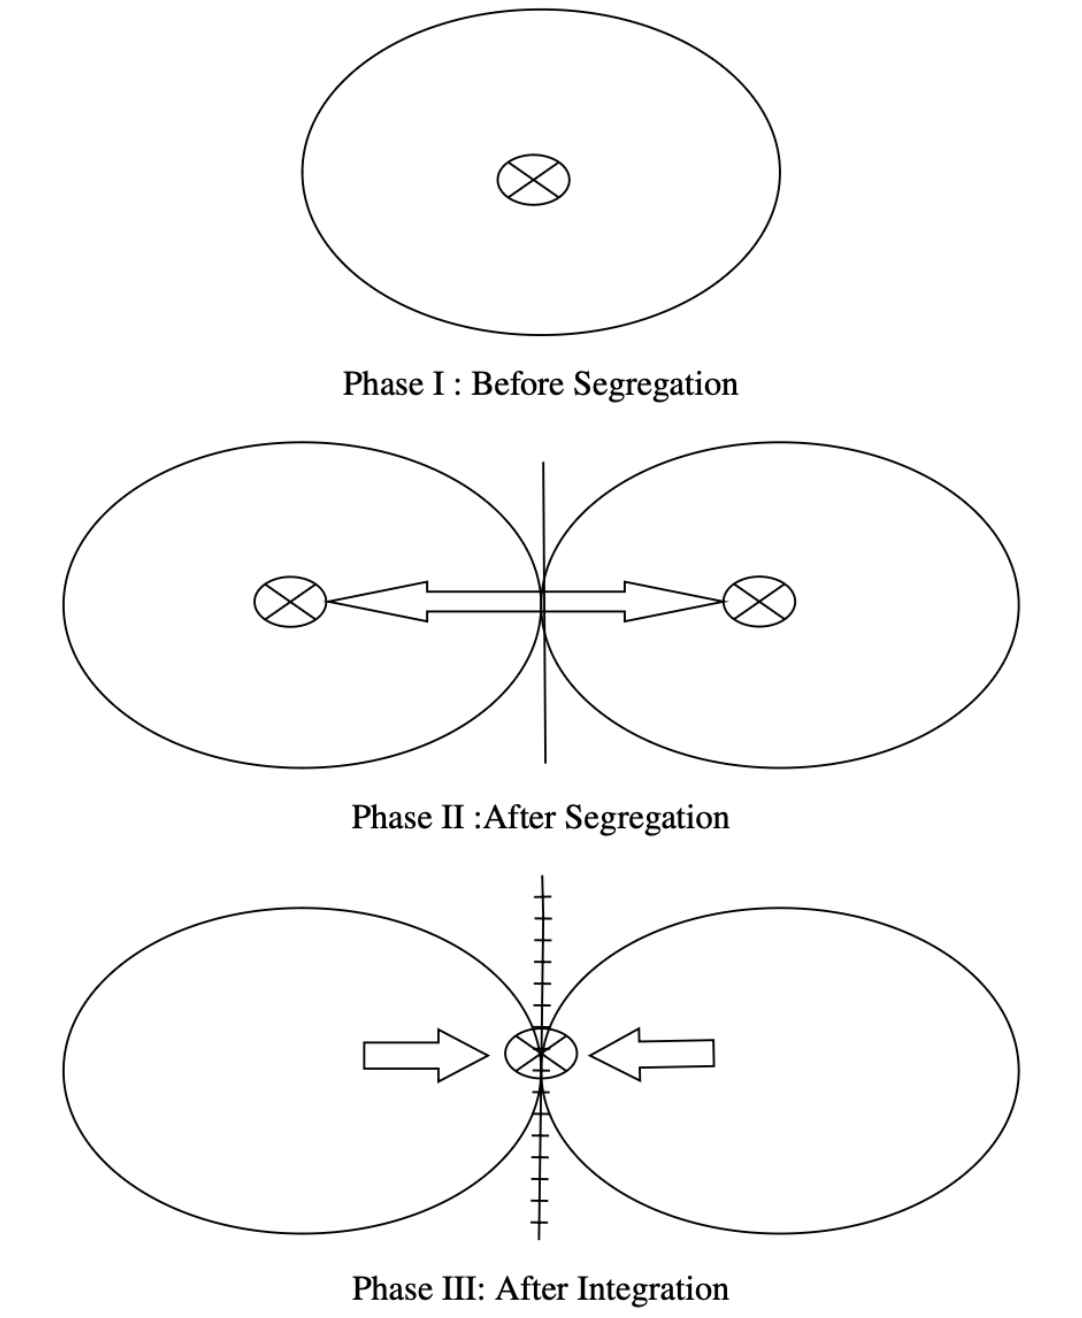
\includegraphics[scale=0.4]{photos/hypoframe.png}
    \floatfoot{ 
\scriptsize \textit{Notes:} Dashed circles in the circles represent 20th historical city centers. Arrays denote in which direction economic activities move. The solid line represents emerged border. The dashed line represents a lifted intra-city or state border.}}
\end{figure}

In 2008, the Schengen Agreement was implemented, which allowed for the elimination of internal border controls. By removing internal border barriers, the Schengen Agreement enabled individuals to travel without passport checks between divided cities. This significantly impacted cross-border economic activities, as it streamlined trade, tourism, and labor mobility. The free movement of people facilitated by the Schengen agreements has fostered closer cooperation and integration between the newly joined countries and the existing EU member states, especially in the context of divided historical cities. 



\subsection{Data}
\par I mainly utilize two datasets. First, I use NASA’s satellite images of Earth at night to measure socio-economic activities at a granular level. Second, I use European business registers to deliver a rich dataset of different types of registered economic entities at a low spatial scale.
\subsubsection{Satellite Nightlights}
\par This paper uses nighttime light data measured by satellites - the only available data source that provides a proxy for the degree of socioeconomic activities since 1992 in Europe at sufficient granularity. In the context of Europe, where comprehensive and fine-grained  data might be challenging to obtain, nighttime light data fill a critical data gap. The availability of consistent and reliable nighttime light data allows researchers to examine socioeconomic patterns, track changes, and explore relationships between human activity and various socioeconomic variables.



\par Researchers often encounter limitations when  obtaining certain types of data, including official statistics such as gross domestic product (GDP), population numbers, and employment rates. These limitations often arise due to constraints related to spatial scale and temporal coverage. Eurostat, the statistical office of the European Union, provides administrative data on economic activities in Europe, but these data are typically aggregated at the NUTS2 and NUTS3 levels, which is unsuitable for fine-grained analysis within cities.


\par In my paper, I aim to overcome these limitations by utilizing satellite-detected nighttime light data. Nighttime light data have been extensively used in economics and are considered one of the most feasible data sources for observing changes in economic or human activities within cities over time. Several studies have measured economic and human activities using the stable nightlights of the Defense Meteorological Satellite Program (DMSP-OLS) in African cities (\citealp{michalopoulos2014national}; \citealp{storeygard2016farther}; \citealp{eberhard2019regional}; \citealp{dreher2019african});  in world cities (\citealp{hodler2014regional}; \citealp{duben2021population}; \citealp{kocornik2020flooded}; \citealp{mamo2019intensive}; \citealp{lessmann2017regional}); in Indian cities (\citealp{gibson2015urban}; \citealp{castello2018higher}); in Indian constituencies (\citealp{baskaran2018women}; \citealp{prakash2019night}); in Barbados beaches (\citealp{corral2017impact}); in Haiti communes (\citealp{mitnik2018bright}); in  OECD countries (\citealp{smith2018left}); in North Korea (\citealp{lee2018international}); and in Indonesian sub-districts (\citealp{heger2019impact}). This dataset has been particularly useful for studying urbanization, economic development, energy consumption, environmental impacts, and other socioeconomic factors. Above mentioned studies have explored a wide range of socioeconomic variables, including GDP estimation, urbanization rates, economic inequality, population distribution, and even public health indicators. The stability and consistent coverage of DMSP-OLS nightlights make it a valuable resource for investigating long-term trends and patterns of economic and human activities at city, national, and global scales.

\par DMSP-OLS captured nighttime images of the Earth from 1993 to 2013. These images were obtained by satellites equipped with sensors that measure the intensity of lights emitted during the night. The resulting raster images have a resolution of 30 arc seconds, which is approximately equivalent to 1x1 km at the equator. This level of detail enables examining changes at a high-resolution spatial level.

\par In the DMSP-OLS raster images, each pixel is assigned a digital number (DN) that represents the intensity of lights in that area. The DN values range from 0 to 63, with 0 indicating no lights and 63 representing the highest concentration of lights. By analyzing these DN values, researchers can quantify the brightness or intensity of nighttime lights and use this information to study various socioeconomic phenomena.  The detailed data are described in \hyperlink{Table 2.A.1}{Table 2.A.1} and \hyperlink{Figure 2.A.1}{Figure 2.A.1}. I built  \href{https://europe-nightlight.shinyapps.io/cities/}{an app} that displays dynamics of remotely sensed nightlights in historically divided border cities.

\par  While other datasets, such as the Visible Infrared Imaging Radiometer Suite (VIIRS) Day/Night Band, have been introduced since 2013 and offer improved capabilities, DMSP-OLS remains the most commonly used dataset for studying long-term trends and relationships between human activity and nighttime lights. Due to the consistent and long-term coverage provided by DMSP-OLS, as well as its relatively high spatial resolution, it has become the common data source for studying long-term changes in nighttime lights and their association with socioeconomic variables.
\subsubsection{Registered Economic Entities}
The concentration of economic activities near historical city centers can be attributed to several channels. These channels can reflect various factors and dynamics that contribute to the spatial organization of economic activities within cities. 

\par  Many historical city centers were established centuries ago, and over time, they became the central hubs of economic and social activities. As a result, businesses catering to consumer needs, such as retail stores, restaurants, cafes, entertainment venues, and tourism-related services, tend to cluster in these areas. This paper account for sectoral specialization, which has not yet been addressed in previous studies. I have collected firm-level data which allows me to understand the dynamics and patterns of economic activities near historical city centers - the specific characteristics and location choices of individual businesses within the city.



\begin{figure}[H] \hypertarget{Figure 2.3}{}
\renewcommand\thefigure{2.3}
\RawCaption{\caption{Economic Entities in Český Těšín
(CZ) - Cieszyn (PL)}}\vskip\captionskip
\floatbox[{\captop}]{figure}[\FBwidth]
    {}
   {
    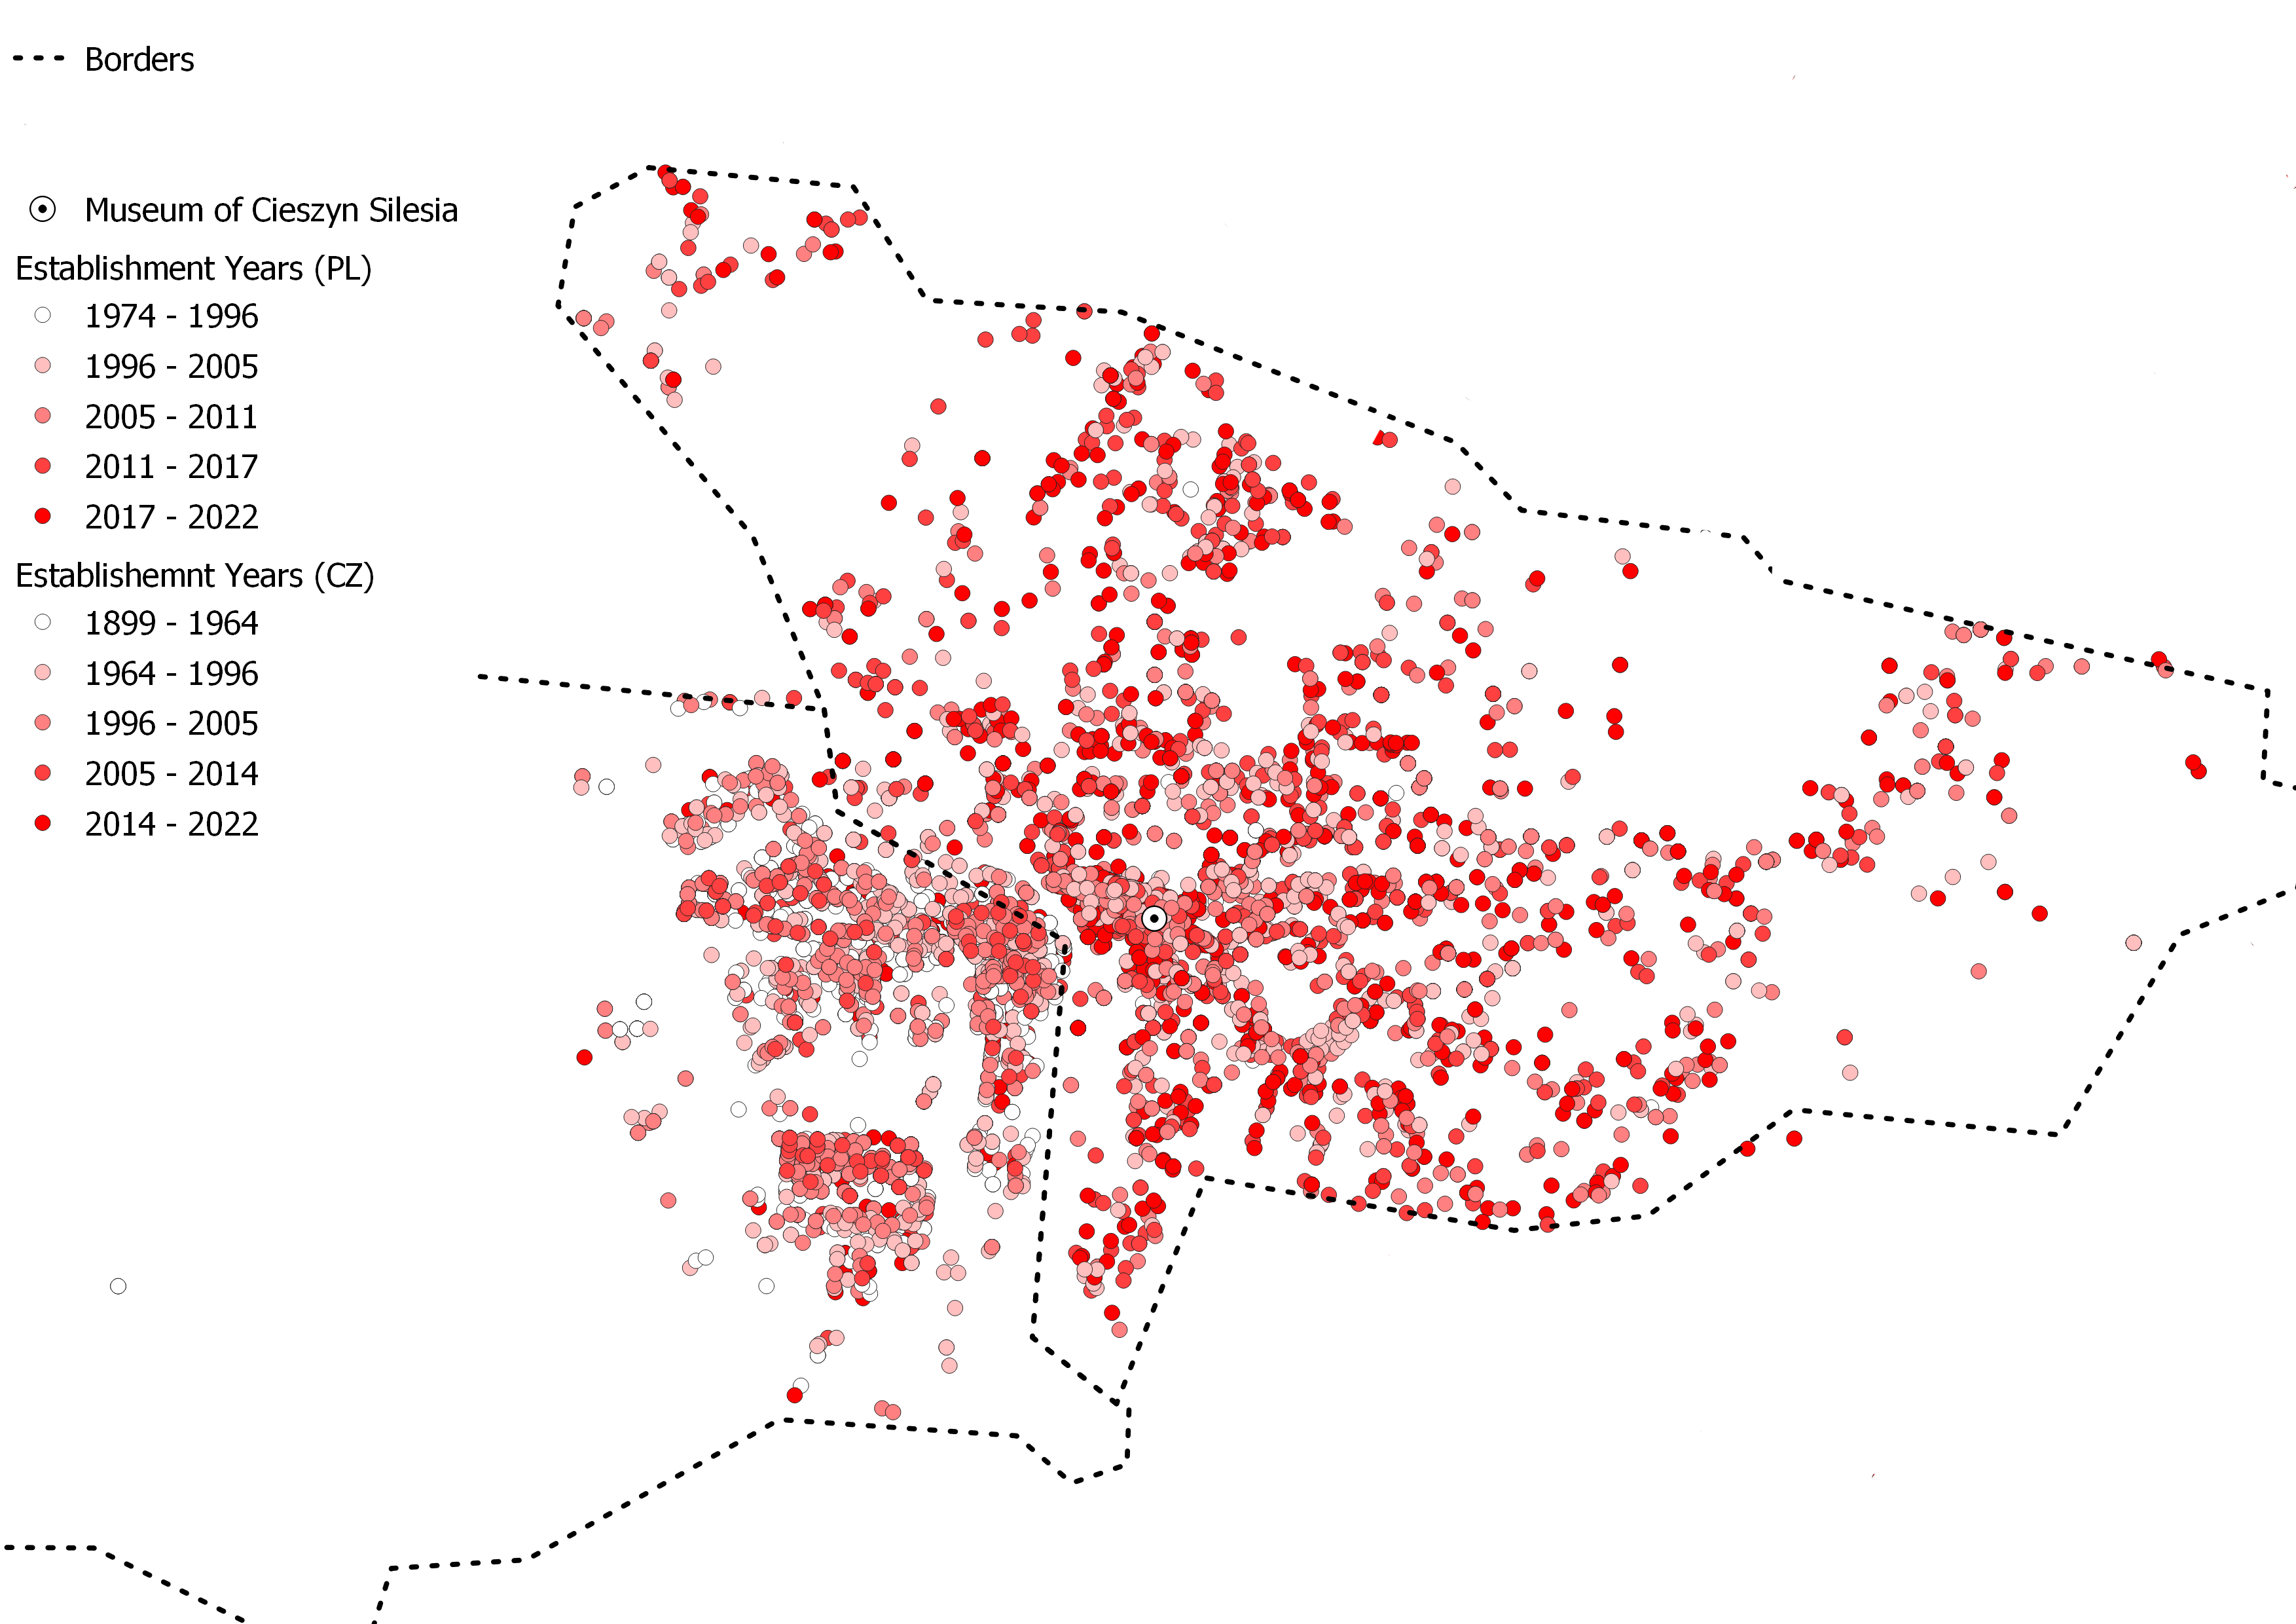
\includegraphics[scale=0.4]{photos/cz_pl.png}
    \floatfoot{ 
\scriptsize \textit{Source:} Author's elaboration in QGIS based on geo-coded Registers Data \\Notes: The map presents the locations and establishment years of economic entities in the divided cities of Cesky Tesin and Cieszyn. Dashed lines represent internal/state borders. Various points show the establishment years of economic entities during 1900-2022. The black-and-white dot denotes pre-war historical city center, identified by the Museum of Cieszyn in Silesia.}}
\end{figure}



 
\par In order to uncover this channel, I use information from registers of economic entities. I constructed the database by bringing together several datasets containing information on about registration of economic entities. I define an economic entity as any legal entity that appears in a public register and is administered by the Ministry of Justice in Czechia, Slovakia, Slovenia, Germany, Poland, Hungary, Estonia, and Latvia. This definition encompasses a broad range of entities, including businesses, corporations, partnerships, and other legally recognized entities involved in economic activities within these countries.

\par My primary focus is on the establishment years of economic entities. The database I have compiled includes information on all legally recorded entities. By collecting data on entries, I can track changes in the economic landscape over time \footnote{National register databases suffer a survival bias, especially for data collected before 1990. Moreover, in some countries, data does not exist, i.e., due to the Soviet Union’s planned market regulations, there were  no registration records before 1990 in Estonia and Latvia.}. 





\begin{figure} \hypertarget{Figure 2.4}{}
\renewcommand\thefigure{2.4}
\centering
\subfigure[NTL in 2002]{\label{}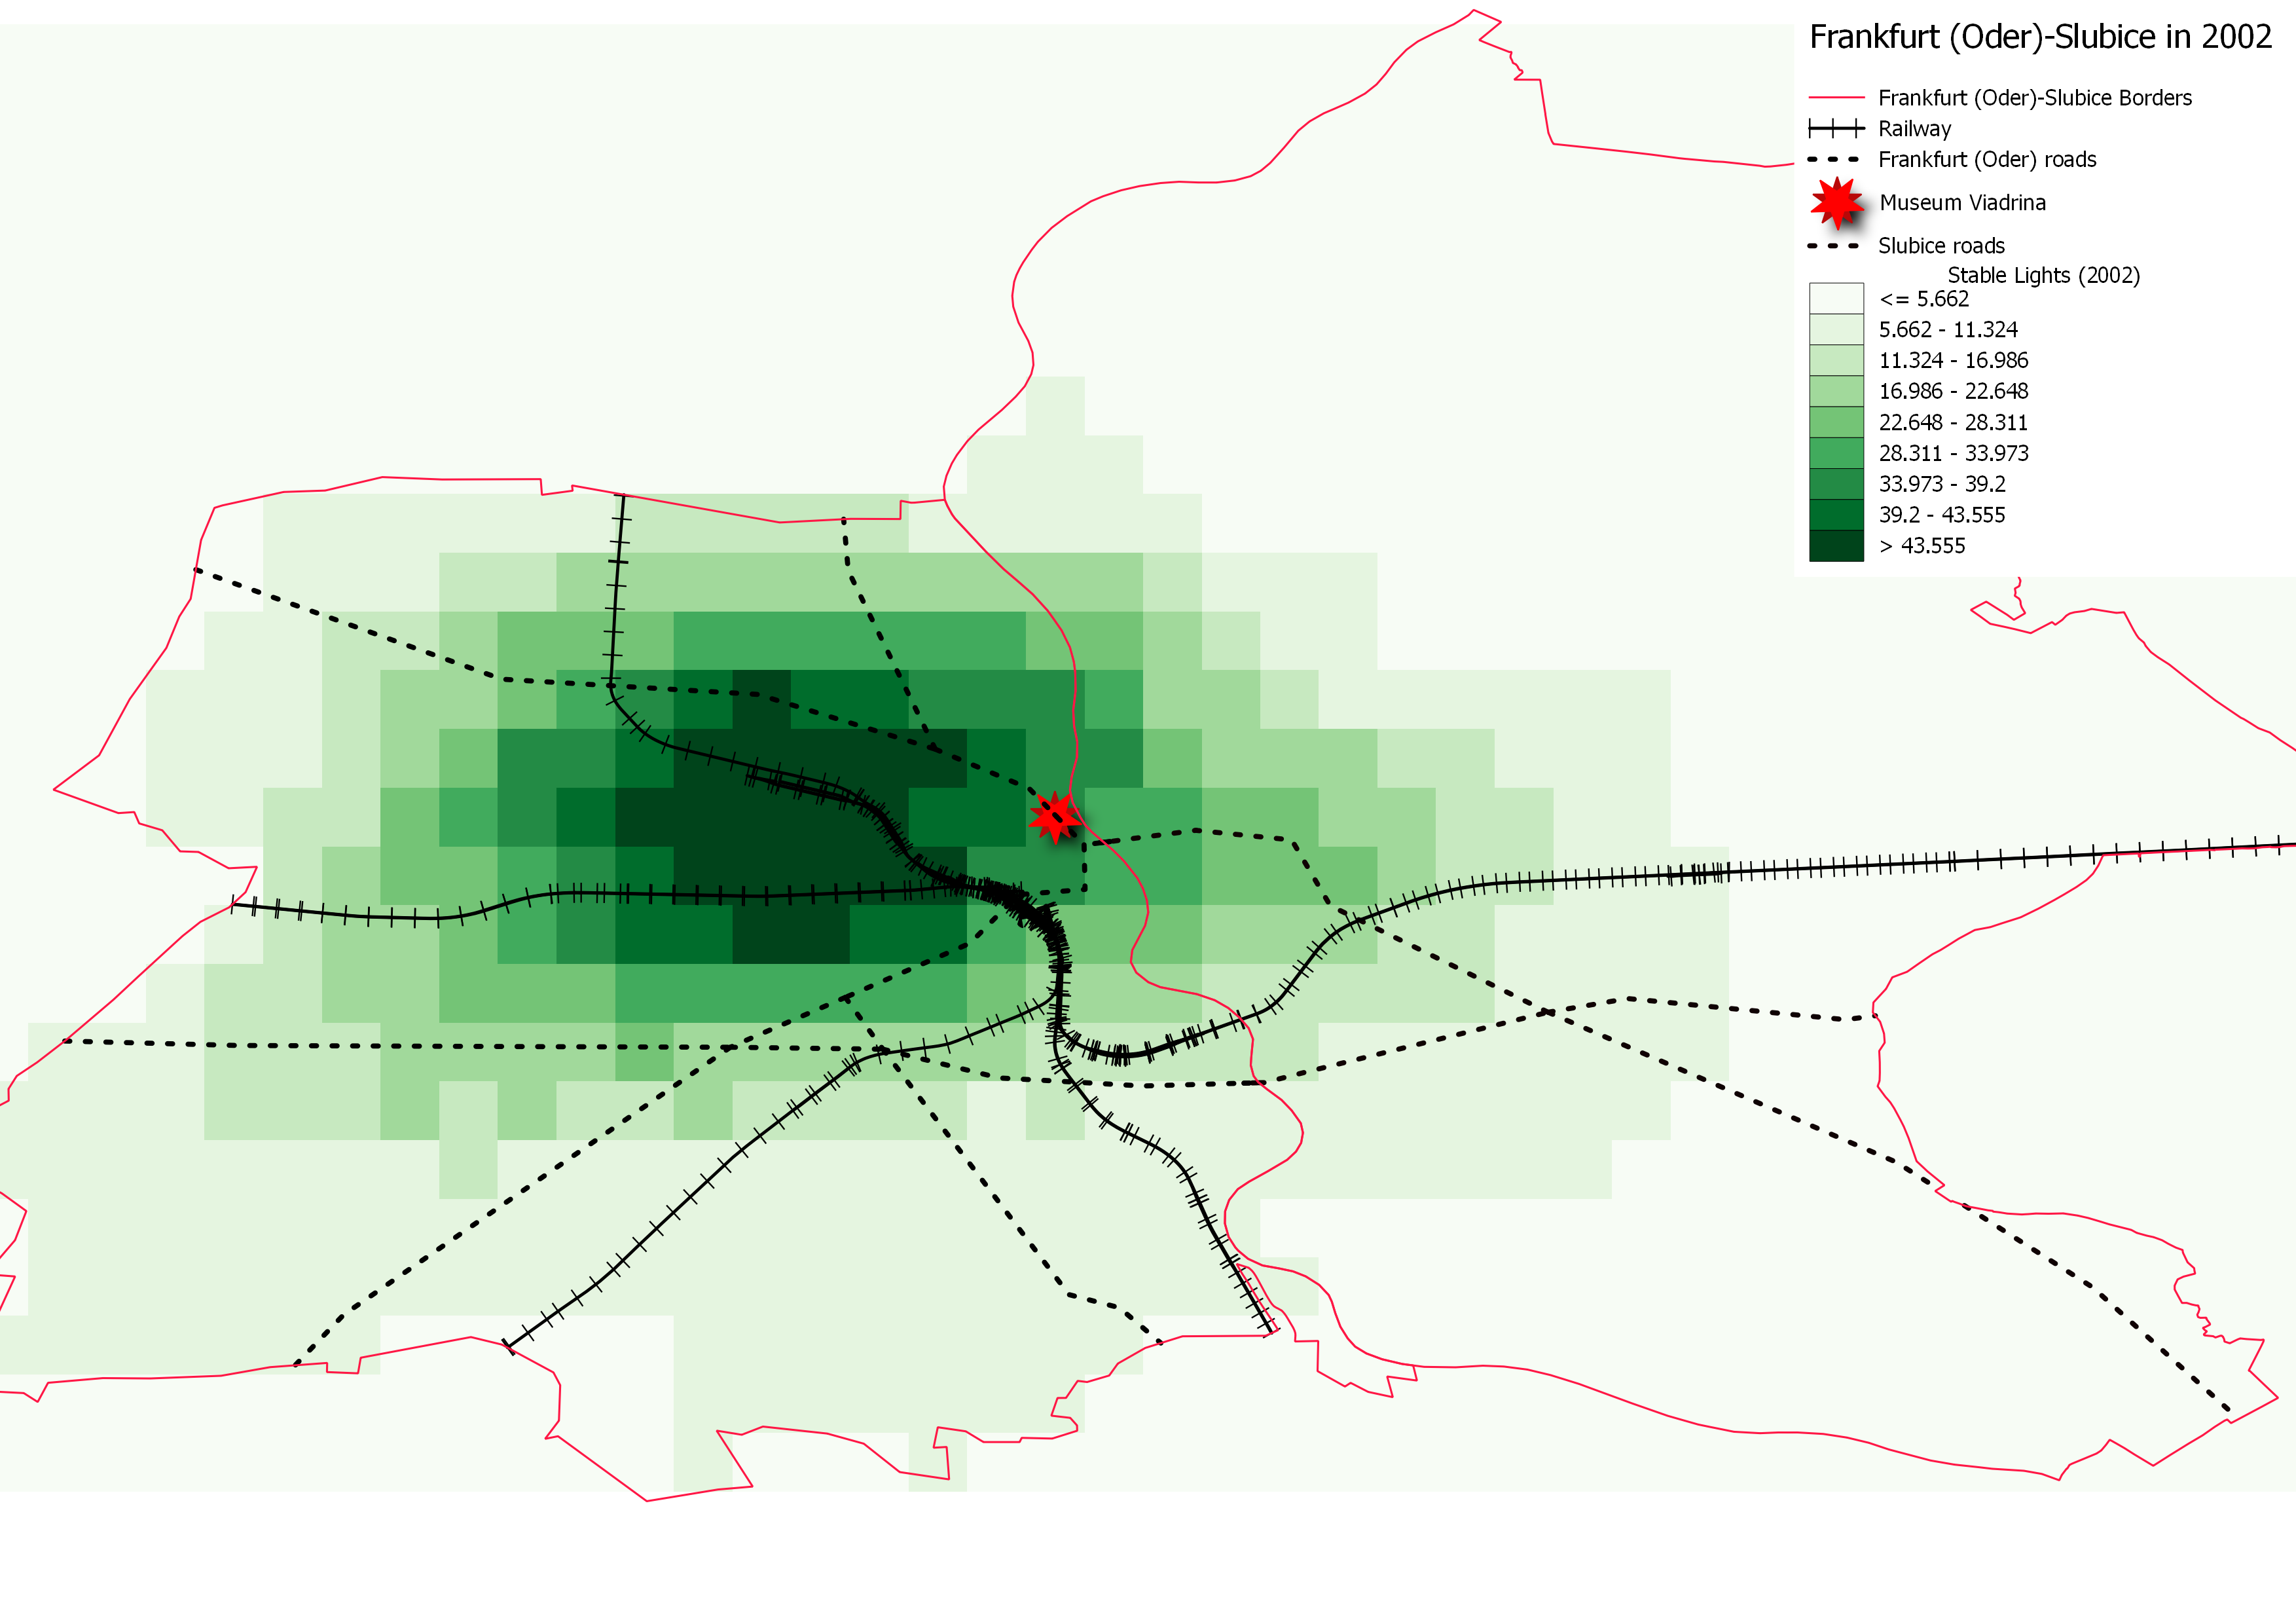
\includegraphics[width=.4\linewidth]{photos/FS2002.png}}\hfill
\subfigure[NTL in 2008]{\label{}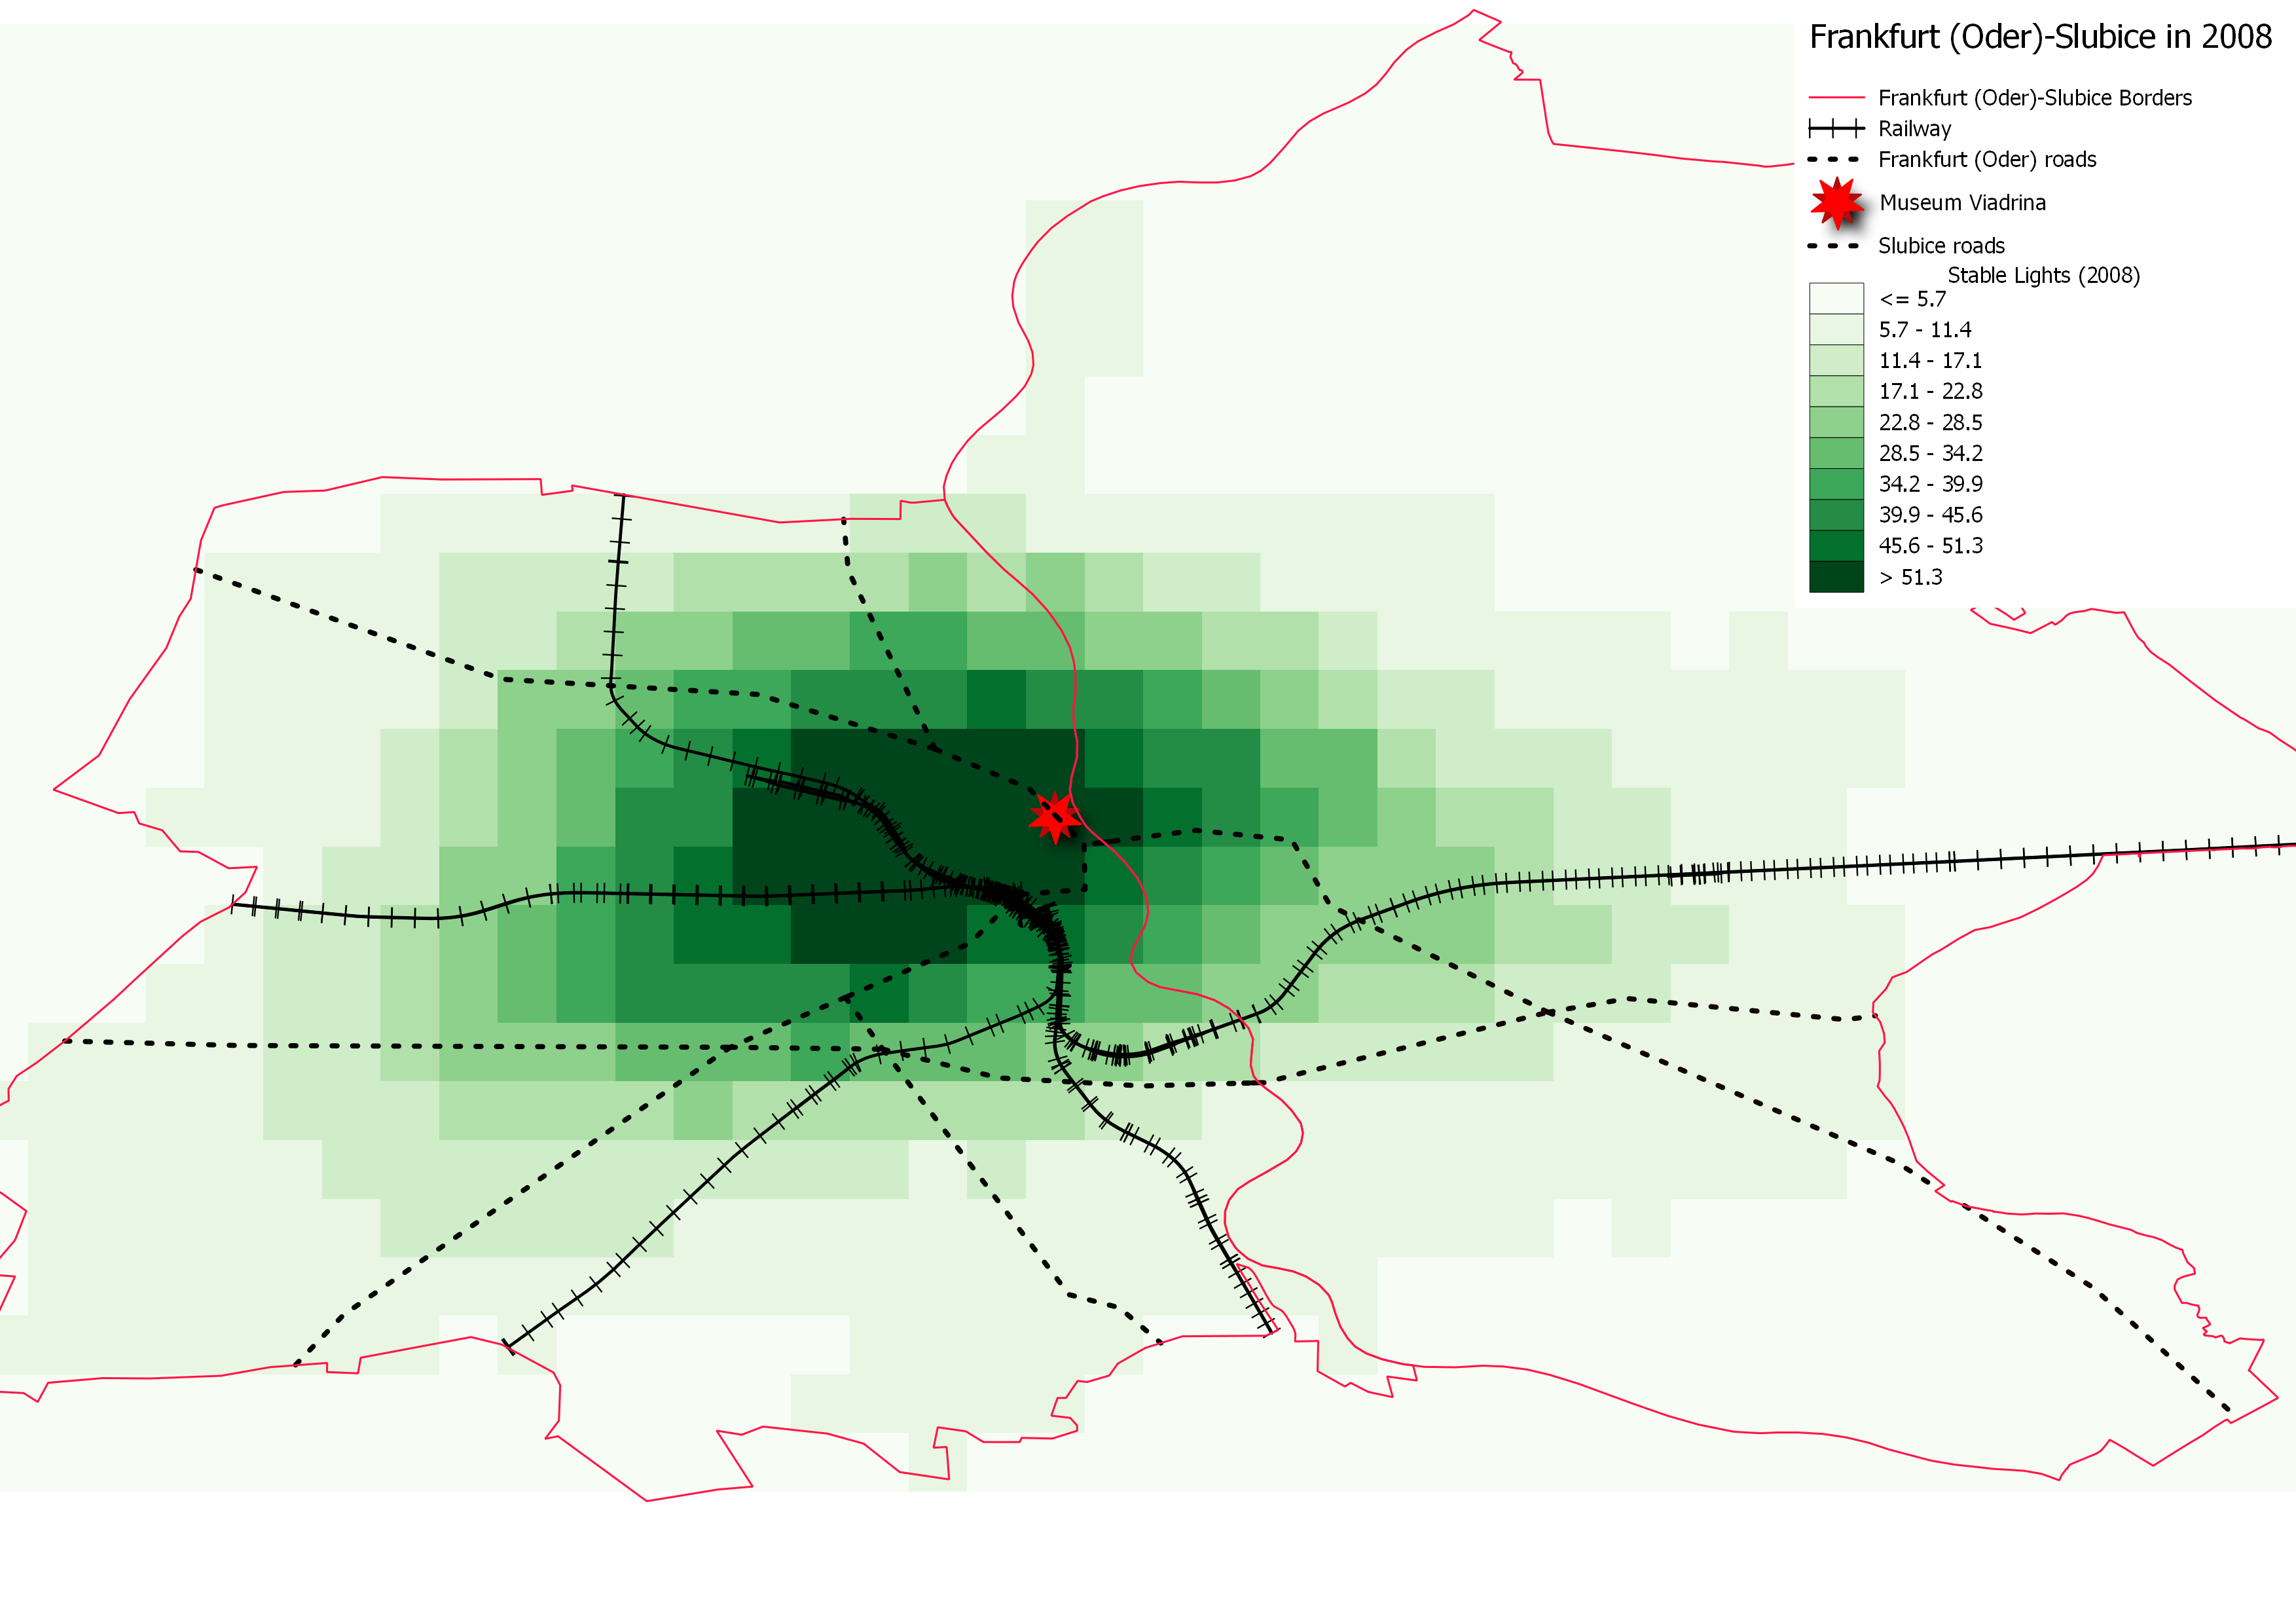
\includegraphics[width=.4\linewidth]{photos/FS2008.png}}\par 
\subfigure[NTL in 2012]{\label{}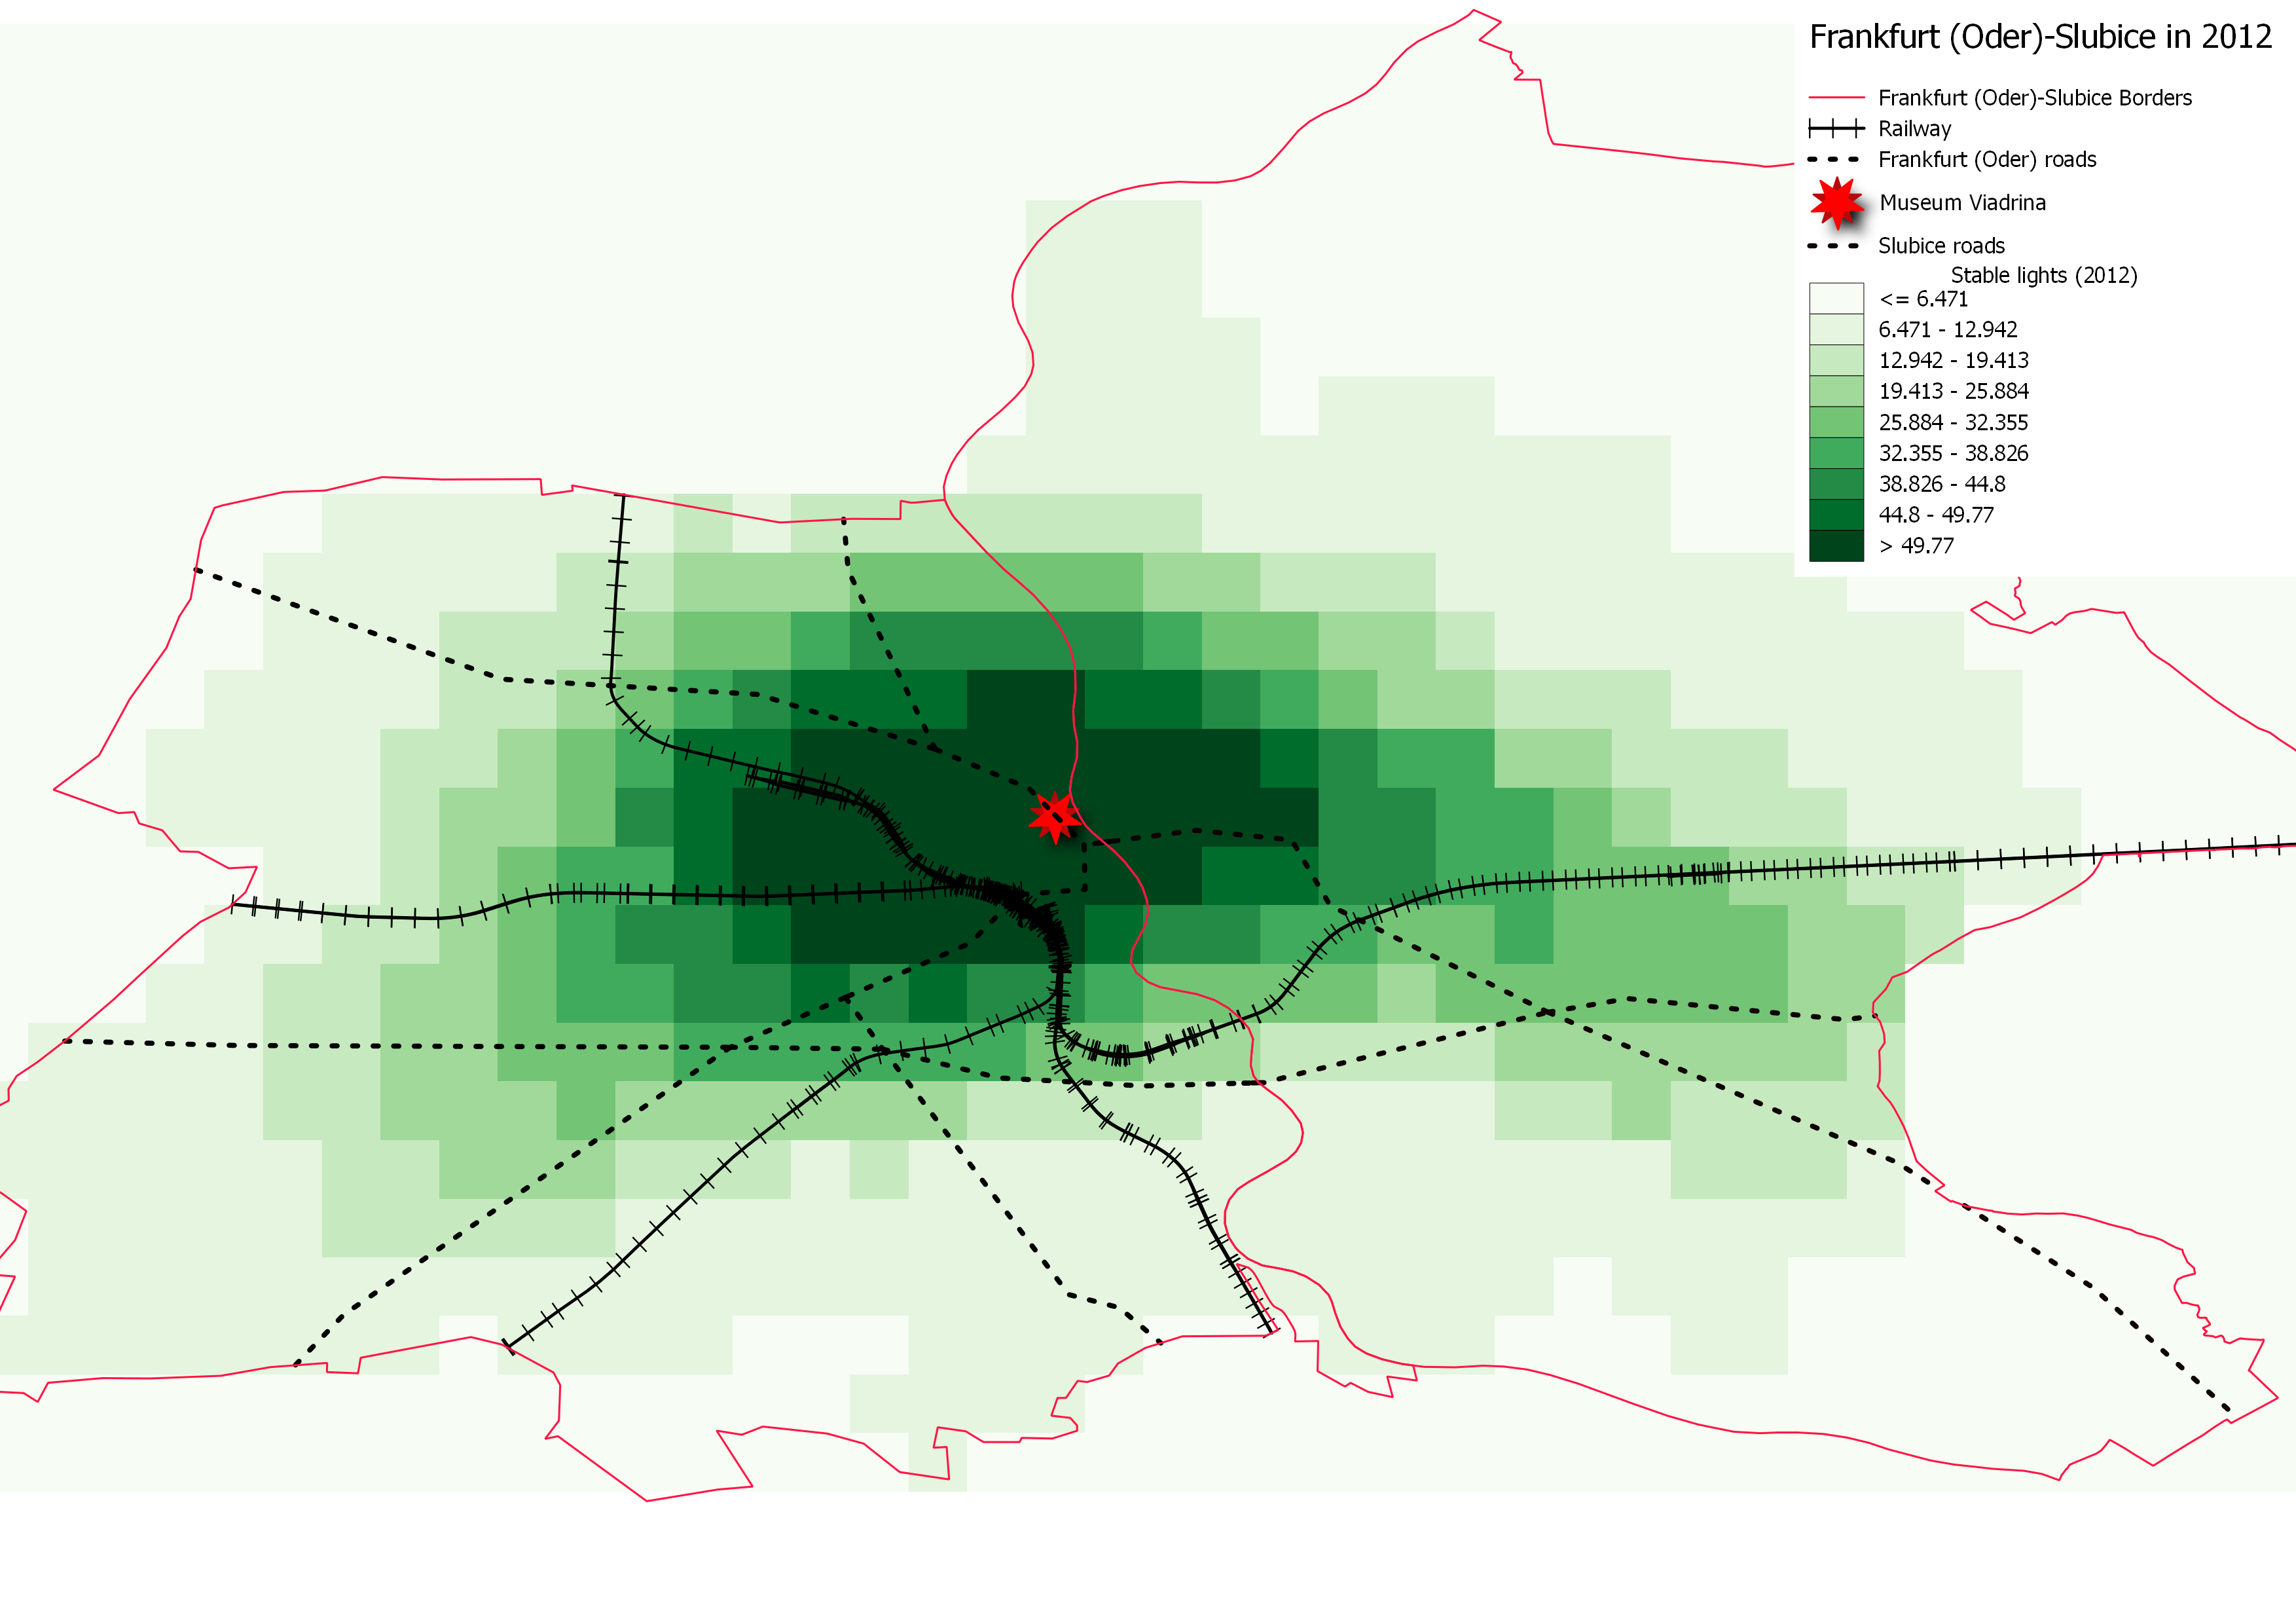
\includegraphics[width=.4\linewidth]{photos/FS2012.png}}
\caption{Nighttime Lights in Divided Cities: Frankfurt (Oder) \& Slubice}
{
 \floatfoot{ 
\footnotesize 
\textit{Source:} Author’s calculations based on DMSP-OLS satellite data. 
\\Map (a) represents DMSP-OLS stable lights in 2002, map (b) represents stable lights in 2008, and map (c) represents stable lights in 2012. On the maps, the dashed lines represent German and Polish road connections. The red star is the historical city center, denoted by  \textit{the Museum of Viadrina}. }}
\end{figure}


\par In \hyperlink{Figure 2.3}{Figure 2.3}, I show an example of locations and establishment years of economic entities in Český Těšín on the Czech side and in its divided city of Cieszyn on the Polish side. I geo-referenced each registered economic entity in the sample in QGIS and Google Earth Pro. The final georeferenced data has information on economic entities, including the establishment years, addresses (e.g., exact addresses with latitude and longitude coordinates), names, and NACE2. For details of data availability on entry dates, NACE2 codes, and coordinates, see  \hyperlink{Table 2.B.1}{Table 2.B.1}. 

\subsection{Empirical Results}
For the initial descriptive and motivational purpose, I illustrate the evolution of nighttime lights in one pair of divided cities: Frankfurt (Oder), Germany, and Slubice, Poland.


\par In \hyperlink{Figure 2.4}{Figure 2.4} map (a), during the pre-intervention period before the borders between Frankfurt (Oder) and Slubice were abolished, economic activities were not concentrated near the Museum Viadrina or the city center area. This suggests that economic activities were dispersed throughout the city.



\par In \hyperlink{Figure 2.4}{Figure 2.4} map (b), after the implementation of the Schengen agreement, which allowed for the free movement of people and goods within the Schengen Area, economic activities became more concentrated near the pre-war historical city center. This indicates that the removal of border restrictions and the increased mobility of people may have contributed to a clustering of economic activities in the pre-division city center.

\par Finally, in \hyperlink{Figure 2.4}{Figure 2.4} map (c), which represents the situation in 2012, after the free movement of Polish workers to Germany became allowed, economic activities grew even more and concentrated near the former historical city center. This suggests that the influx of Polish workers led to further economic concentrations near the historical city center.



\par Overall, these three maps demonstrate a shift in economic activities from a dispersed pattern to a more concentrated one near the historical city center over time. This transformation can be attributed to the abolition of borders, which facilitated increased mobility and economic integration between the divided cities.

\par Since \hyperlink{Figure 2.4}{Figure 2.4} hints to the concentration of economic activities near the city center, I empirically test the following baseline model: 

\begin{equation} 
\renewcommand\theequation{2.1}
\begin{split}
Log(DN)_{it}=&\beta_1+\beta_2 Integration_{t}+ \beta _{3} HCTR_{i} + \beta_4  Integration_{t}\times HCTR_{i}+\epsilon_{it}
\end{split}
\end{equation}
where $i$ denotes a unit of analysis at 1x1 \textit{km} grid cell; $ Log(DN_{it})$ represents the digital number of stable lights (DN) -  a proxy of local socioeconomic outcomes in grid cell $i$ at time $t$; $HCTR_{i}$ measures the proximity  to a historical city center, from grid cell $i$ to historical center and is standardized based on the geographical size of the city; $Integration_{i,t}$ is a indicator variable which represents stepwise abolishing of borders: is a dummy variable taking a value of one after 2004 (EU Enlargement), and zero otherwise and is a dummy variable taking a value of one after 2008 (Schengen), and zero otherwise; the key interaction coefficient explains how NTL grew in  areas close to historical centers after border barriers were removed; $\epsilon_{it}$ is an error term. Standard errors are  heteroskedasticity-autocorrelation (HAC) robust in all specifications.

\par I standardize historical centers based on the geographical size of each city at LAU-2 level: 
\begin{equation*}
StandardizedDistance_i=\frac{Distance_{ij}}{CitySize_i} 
\end{equation*}

Here, $Distance_{ij}$ denotes the distance from pixel $i$ to historical center $j$, while $CitySize_i$ represents the population density of the city where pixel $i$ is situated. The term $StandardizedDistance$ refers to the distance of each pixel $i$ to historical centers, which has been standardized. This standardization enables the creation of comparable distances to historical centers irrespective of the city's size. For instance, the distance to the historical center in Cesky Tesin can be reasonably compared to the distance to the historical center in Frankfurt (Oder).

Upon computing the standardized distance for each pixel within the dataset, I proceeded to determine the proximity to historical centers using the subsequent formula:

\begin{equation*}
    ProximityToHCTR_i=-StandardizedDistance_i
\end{equation*}

Where $ProximityToHCTR_i$ indicates the distance measured in kilometers from the historical city centers.

\par The European integration facilitated greater access to non-tradable goods and services on the other side of the border. The increased ease of movement across borders allowed people to take advantage of the proximity of pre-division historical centers and consume goods and services available in those areas.

\par By reducing and removing barriers to cross-border movement, people living near the border could easily access nearby zones with pre-division historical centers and consume goods and services that were locally available but might have been more convenient or attractive in terms of price, quality, or variety. Such cross-border consumption could influence location decisions and economic activity patterns within divided historical cities. Firms might have been attracted to areas near pre-division historical centers due to the increased demand generated by the movement of people seeking local non-tradable goods and services. 





\begin{table}[H]  \hypertarget{Table 2.2}{}
\renewcommand\thetable{2.2}
\centering
\footnotesize
\def\sym#1{\ifmmode^{#1}\else\(^{#1}\)\fi}
\caption{The Effect of Stepwise Integration on Nightlights in Divided Cities}


\begin{tabular}{l*{3}{D{.}{.}{-1}}}
\toprule
                    &\multicolumn{1}{c}{(1)}         &\multicolumn{1}{c}{(2)}         &\multicolumn{1}{c}{(3)}         \\

                
                    & Log(NTL)& Log(NTL) &Log(NTL)\\ 
                
\midrule
European Union&       0.188\sym{***}&       0.216\sym{***}&                     \\
                    &     (0.016)         &     (0.016)         &                     \\
\addlinespace
European Union $\times$ HCTR &      -0.226\sym{*}&      -0.060\sym{**}&                     \\
                    &     (0.024)         &     (0.026)         &                     \\
\addlinespace
Schengen     &       0.199\sym{***}&                     &       0.171\sym{***}\\
                    &     (0.016)         &                     &     (0.016)         \\
\addlinespace
Schengen $\times$ HCTR&       0.277\sym{***}&                     &       0.108\sym{***}\\
                    &     (0.027)         &                     &     (0.029)         \\
\midrule
N        &       74729         &       74729         &       74729         \\
\(R^{2}\)           &       0.233         &       0.231         &       0.232         \\
\bottomrule
Time Span & 1992-2013 & 1992-2013  & 1992-2013 \\
\toprule
&&&\\
Treatment Years & & 2004-2013 & 2008-2013\\
\toprule
    &&&\\
    \bottomrule
Year FE  (1992-2013)      &        \checkmark          &        \checkmark          &        \checkmark          \\
Satellite FE (5 years interval)      &        \checkmark          &        \checkmark          &        \checkmark          \\
Pixel FE  (1x1 km)     &        \checkmark          &        \checkmark          &        \checkmark          \\
\bottomrule
{\floatfoot{\scriptsize \textbf{Notes}: \textit{Estimation method:} panel fixed effects. \textit{Dependent variable:} Log(NTL) is log transformed NTL luminosity. Robust standard errors in parentheses.  (⁎) (⁎⁎) (⁎⁎⁎) denotes statistical significance at the (10) (5) (1) percent level. Robust standard errors in parentheses. HCTR is in proximity to historical centers and is standardized based on the geographical size of the city. \textit{Source:} Author's calculations.}}\\
\end{tabular}
\end{table}







\begin{table}[H]  \hypertarget{Table 2.3}{}
\renewcommand\thetable{2.3}
\centering
\footnotesize
\def\sym#1{\ifmmode^{#1}\else\(^{#1}\)\fi}
\caption{ The Effect of European Division and Integration on Establishments}
\begin{tabular}{l*{4}{D{.}{.}{-1}}}
\toprule
                    &\multicolumn{1}{c}{(1)}         &\multicolumn{1}{c}{(2)}         &\multicolumn{1}{c}{(3)}         &\multicolumn{1}{c}{(4)}         \\
\toprule
    &&&\\
                    & \# firms &  \# firms & \# firms & \# firms\\ 
\midrule

Division            &       -9.437  &     -23.103\sym{***} &                     &                     \\
                    &     (4.968)         &     (9.405)         &                     &                     \\
\addlinespace
Division $\times$ HCTR&      -2.252\sym{**}         &      -3.351\sym{***} &                     &                     \\
                    &     (1.827)         &     (1.662)         &                     &                     \\

\addlinespace
European Union                &      32.911\sym{*}&                     &      28.321\sym{***}&                     \\
                    &     (2.892)         &                     &     (3.521)         &                     \\
\addlinespace
European Union $\times$ HCTR    &      -0.023         &                     &       0.037         &                     \\
                    &     (0.245)         &                     &     (0.270)         &                     \\
Schengen            &      -5.077         &                     &                     &      27.362\sym{}\\
                    &     (3.380)         &                     &                     &     (1.872)         \\
\addlinespace
Schengen $\times$ HCTR  &       1.531\sym{**}&                     &                     &       1.648\sym{***}\\
                    &     (0.414)         &                     &                     &     (0.490)         \\
\addlinespace

\midrule
N of blocks       &        3101         &        3101         &        1731         &        3101         \\
N of firms       &        42448         &        42448         &        32327         &        42448         \\
\(R^{2}\)           &       0.240         &       0.143         &       0.243         &       0.239         \\
\bottomrule
Time Span & 1945-2020 & 1980-2020  & 1945-2008 & 1945-2020 \\
\toprule
&&&\\
Treatment Years &  & 1980-1990 & 2004-2008 & 2008-2020\\
\bottomrule
Year FE (1900-2020)       &        \checkmark   &        \checkmark        &        \checkmark          &        \checkmark          \\
Block FE   (500x500meters)    &        \checkmark  &        \checkmark         &        \checkmark          &        \checkmark          \\
\bottomrule

N of firms       &        42448         &        42448         &        32327         &        42448         \\
N of firms       &        42448         &        42448         &        32327         &        42448         \\
\bottomrule

{\floatfoot{\scriptsize \textbf{Notes}: \textit{Estimation method:} panel fixed effects. \textit{Dependent variable:} is \#firms (number of firms) -  total number of firms based on establishment years in 500x500m grid/block.  (⁎) (⁎⁎) (⁎⁎⁎) denotes statistical significance at the (10) (5) (1) percent level. Robust standard errors in parentheses. HCTR is proximity to historical centeres and is standardized based on the geographical size of the city. The sample includes 11 cities: České Velenice, Český Těšín, Cieszyn, Gorizia, Nova Gorica, Komárno, Komárom, Słubice, Valga, and Zgorzelec. This selection was constrained by the lack of NACE classifications or precise locational data for firms in other cities. Overall, the analysis includes 42,448 firms out of a total of 54,669. \\\textit{Source:} Author's calculations.}}\\
\end{tabular}
\end{table}

\par However, on the other hand, in the presence of low trade costs within a city, changes only in goods mobility may have a limited impact on firm location decisions within the city. When trade costs are already low, changes in goods mobility are unlikely to have a significant influence on firm location decisions within a city. \hyperlink{Table 2.2}{Table 2.2} in column (2) shows that economic activities are not concentrated in a close radius to historical centers, indicating that other factors play a more prominent role in determining firm location towards historical city centers. 





\par After discussing the results of the EU analysis, it is worthwhile to shift the focus to the 2008 Schengen enlargement. In \hyperlink{Table 2.2}{Table 2.2} in columns (1) and (3), the results indicate that in areas near the former historical city centers, there is an approximate increase of 10 percentage points in annual NTL radiance at the 1x1km grid cell level. This finding suggests that these areas experienced a relative increase in economic activities, as represented by the increase in nighttime light intensity, compared to other zones. The analysis demonstrates that the areas in proximity to historical city centers exhibited a stronger economic performance relative to their respective pre-Schengen (\textit{borderless} travel area) levels. This finding suggests that the removal of border restrictions within the Schengen area has contributed to increased economic activity and development in these areas. These results provide evidence of the economic impact of the Schengen agreement inside the divided city and highlight the significance of proximity to historical city centers.

\par The increased economic activity near historical city centers can have positive spillover effects on the surrounding zones as well. The concentration of economic activities in these areas can lead to job creation and investment opportunities, further stimulating the labor and employment economy.




\par To further enhance my analysis, I geocoded economic entities registered in divided historical cities. I have created a three-way panel dataset that captures the establishment of firms within 500m x 500m blocks over a span of the century 1900-2020. This dataset includes information on the firms, the blocks in which they are located, and the corresponding year of establishment. So I can identify clusters of firm establishments within certain blocks and identify periods of rapid growth or decline in firm formation within specific blocks. I run the fixed effects models on my three-way panel dataset:



\begin{equation} 
\renewcommand\theequation{2.2}
\begin{split} 
\# firms_{i,b,t}=&\beta_1+\beta _2 Division_{i,b,t}+ \beta_{3} HCTR_{i,b} +\beta_4 Division_{i,b,t}\times HCTR_{i,b}+\epsilon_{i,b,t}
 \end{split}
\end{equation}

\begin{equation}
\renewcommand\theequation{2.3}
\begin{split}
\# firms_{i,b,t}=&\beta_1+\beta _2 Integration_{i,b,t}+ \beta_{3} HCTR_{i,b} +\beta_4 Integration_{i,b,t}\times HCTR_{i,b}+\epsilon_{i,b,t}
    \end{split}
\end{equation}
\par 


Where subscript $i$ denotes a registered economic entity; subscript $b$ denotes a 500x500m block; and subscript $t$ denotes time; variable $\# firms_{i,b,t}$ is constructed from the total number of firms in block $b$ established at time $t$; $HCTR_{i}$ measures the proximity  to a historical city center, from grid cell $i$ to the historical center and is standardized based on the geographical size of the city; 



$Division_{i,b,t}$ represents the time period of interest when division was prevalent and is a dummy variable that takes a value of 1 for the time period from 1945 to 1990 when cities were  segregated politically, institutionally, and economically; $Integration_{i,b,t}$  represents the stepwise removal of a border and is a dummy variable that takes a value of 1 during the period of 2004-2008 when countries became members of the European Union (EU); $Integration_{i,b,t}$ is a dummy variable that takes a value of 1 during the period of 2008-2020 when countries became members of the Schengen Agreement; interactions express the difference in the number of economic entities established in blocks close to pre-war centers compared to remote blocks during the division and after integration, respectively; $\epsilon_{i,b,t}$ is an error term.

\par Overall, the consistency between the regression results in \hyperlink{Table 2.3}{Table 2.3} using registered economic entities and \hyperlink{Table 2.2}{Table 2.2} using remotely sensed nightlight data strengthens my findings. 

\par The results of the estimated models indicate that there was a concentration of newly established economic entities away from the pre-war historical centers following the division of historical border cities between 1945 and 1990. The concentration of newly established economic entities away from the pre-war historical centers suggests that other areas or regions experienced increased economic activities following the division. Furthermore, establishing new borders and the physical separation of historical border cities have disrupted the flow of goods, services, and people between the pre-war historical centers and the newly formed cities. This disruption created barriers for businesses operating in the pre-war historical centers. In \hyperlink{Table 2.3}{Table 2.3}, in columns (1) and (2), I show that disruptions led to the establishment of economic entities in areas outside the historical centers.

\par Furthermore, in \hyperlink{Table 2.3}{Table 2.3}, column (1) and (3) demonstrates that there was no significant change in the concentration of newly established entities after the political and economic union, specifically after the 2004 Eastern enlargement. This finding suggests that the expansion of the union did not lead to a notable shift in the spatial concentration of economic entities near the historical city center. 

\par However, in \hyperlink{Table 2.3}{Table 2.3} columns (1) and (4) show that it appears that, on average, for every block (500x500m) closer to the historical city center, there is an average increase of 2 firms in the area. This suggests that the ability for individuals to freely move and interact across formerly divided cities plays a crucial role in shaping the spatial distribution of economic entities. 

\begin{table}[H]
\hypertarget{Table 2.4}{}
\renewcommand\thetable{2.4}
\centering
\footnotesize
\def\sym#1{\ifmmode^{#1}\else\(^{#1}\)\fi}
\caption{Language and Cultural Similarities}
\begin{tabular}{l*{4}{D{.}{.}{-1}}}
\toprule
                    &\multicolumn{1}{c}{(1)}         &\multicolumn{1}{c}{(2)}         &\multicolumn{1}{c}{(3)}         &\multicolumn{1}{c}{(4)} \\
\midrule
& Lexical Similarity&No Lang. Barrier&Cesky Tesin& Ciezsyn\\
\midrule
Schengen            & 22.925\sym{***} &      30.734\sym{***}&      55.305\sym{**} &      34.307\sym{***}\\
                   & (5.575)&     (3.724)         &    (19.561)         &     (2.538)         \\
\addlinespace
Schengen $\times$ HCTR  &  0.545  &       2.001\sym{***}&       8.251\sym{*}         &       3.643\sym{***}\\
              & (0.872)      &     (0.660)         &     (4.526)         &     (1.105)         \\
\addlinespace
Schengen $\times$ Lexical &  13.657&       &  &\\
&(14.410) &&\\
\addlinespace
Schengen$\times$ Lexical $\times$ HTCR & 4.646\sym{**}  &     &  &\\
&( 2.589) &&\\
  
\midrule
Observations   &  3101   &        1329         &         188         &         434         \\
\(R^{2}\)       &   0.240  &       0.358         &       0.620         &       0.663         \\
\bottomrule
Year FE  (1900-2020)    &  \checkmark  &       \checkmark         &       \checkmark          &       \checkmark         \\
Block FE  (500x500meters)   &  \checkmark   &      \checkmark         &       \checkmark          &      \checkmark         \\
\bottomrule
{\floatfoot{\scriptsize \textbf{Notes}: \textit{Estimation method:} panel fixed effects. \textit{Dependent variable:} is \#firms (number of firms) -  total number of firms based on establishment years in 500x500m grid/block.  (⁎) (⁎⁎) (⁎⁎⁎) denotes statistical significance at the (10) (5) (1) percent level. Robust standard errors in parentheses. HCTR is proximity to historical centers and is standardized based on the geographical size of the city. \textit{Source:} Author's calculations.}}\\
\end{tabular}
\end{table}



\subsection{Main Channels and Disscusions}
\par In addition to the free movement of people,  cultural and linguistic factors can contribute significant roles in shaping economic activities and concentration in divided cities. 

\par Language is deeply tied to culture and plays a crucial role in shaping economic dynamics. Also, language serves as an important tool for cultural understanding and market adaptation, especially in cross-border areas (\citealp{european2015cross}).




\par Firms can connect with more customers and take advantage of potential opportunities in cross-border regions if residents speak similar languages on both sides of the border. It is important to note that if such companies are located near historical centers in divided cities, they may have a unique opportunity to access and cater to both local and foreign markets, markets of similar language, on each side of the border. A market of similar language refers to a market where the majority of the population shares a common language or where linguistic similarities exist among the population.

\par  I investigate the linguistic proximity between divided cities and show whether cities sharing a common or similar language with their neighbors experience stronger economic concentrations near historical city centers.  



\par To proxy language and culture similarities, I use the lexical similarity coefficients from \href{https://www.ethnologue.com}{Ethnologue} website. These estimates indicate that approximate percentages of what extent the vocabulary items in language A and language B may have similarities or shared roots. The Czech-Austrian  similarity estimate is 0.1; Czech-Polish is 0.6; German-Polish is 0.2; Italian-Slovenian is 0.2; Hungarian-Slovakian is 0.1; Estonian-Latvian is 0.5. Low and high coefficient implies that there is limited shared vocabulary and a significant overlap in vocabulary  between the two languages, respectively.


\par In addition to lexical similarity coefficients, I use cross-border cooperation (CBC) survey, which represents respondents' perceptions of what extent the language and cultural differences pose major problems in the cooperation between Country A (domestic) and the cross-border Country B (foreign). The wording of the question I focus on in the survey is: Thinking about the cooperation between (Country A) and [Cross-Border Country B], to what extent are language differences \& cultural differences a  major problem? I have calculated the share of respondents who responded that language, and cultural differences are major problems with foreign cross-border areas (see \hyperlink{Table 2.C.1}{Table 2.C.1}). 


\par Based on \hyperlink{Table 2.4}{Table 2.4} column 1, it appears that cities with higher lexical similarity coefficients tend to experience a concentration of firms near historical city centers after the abolition of all types of borders in 2008. Specifically, I show that  the number of newly created firms is growing by five within a 500x500-meter radius close to the pre-division center after implementing Schengen policies.

\par Moreover, in \hyperlink{Table 2.4}{Table 2.4}, in columns 2 and 3, I show that proximity to a former historical city center matters more in cities where citizens think that language and cultural differences are not a major barrier to cooperation with their cross-border area. For example,  Czech and Polish both languages belong to the West Slavic branch of the Slavic language family, which means they have a common linguistic heritage. In \hyperlink{Table 2.4}{Table 2.4} columns 4 and 5, I show that the average number of firms established based on their proximity to a historical center (within 500m x 500m blocks) is growing roughly by 8 in Cesky Tesin and by 4 in Ciezsyn after 2008. 


%G H I J P Q R S
% A K L M N O

\begin{table}[H]  \hypertarget{Table 2.5}{}
\renewcommand\thetable{2.5}
\centering
\footnotesize
\def\sym#1{\ifmmode^{#1}\else\(^{#1}\)\fi}
\caption{Firms Creation by Sector in Divided Cities, 1900-2022}
\begin{tabular}{l*{3}{D{.}{.}{-1}}}
\toprule
            &\multicolumn{1}{c}{(1)}&\multicolumn{1}{c}{(2)}\\
            &\multicolumn{1}{c}{Consumer Oriented Firms}&\multicolumn{1}{c}{Producer Oriented Firms}\\
\hline
Schengen        &       12.63         &       5.019         \\
            &     (10.92)         &     (5.263)         \\
[1em]
Schengen X HCTR &       0.691\sym{**}  &      0.0395         \\
            &     (0.306)         &     (0.147)         \\
\hline
\(N\)       &        1693         &        1693         \\
Year FE       &     \checkmark            &        \checkmark         \\
Block FE       &        \checkmark         &        \checkmark         \\


\bottomrule
{\floatfoot{\scriptsize \textbf{Notes}: \textit{Estimation method:} panel fixed effects. \textit{Dependent variable:} is \#firms (number of firms) -  total number of firms based on establishment years in 500x500m grid/block.  (⁎) (⁎⁎) (⁎⁎⁎) denotes statistical significance at the (10) (5) (1) percent level. Robust standard errors are in parentheses. HCTR is in proximity to historical centers and is standardized based on the geographical size of the city. Consumer-oriented firms are classified into G (Wholesale and Retail Trade; Repair of Motor Vehicles and Motorcycles), H (Transportation and Storage), I (Accommodation and Food Service Activities), J (Information and Communication), P (Education), Q (Human Health and Social Work Activities), R (Arts, Entertainment, and Recreation), and S (Other Service Activities). Producer-oriented firms are classified into A (Agriculture, Forestry, and Fishing), K (Financial and Insurance Activities), L (Real Estate Activities), M (Professional, Scientific, and Technical Activities), N (Administrative and Support Service Activities), and O (Public Administration and Defence; Compulsory Social Security). \textit{Source:} Author's calculations.}}\\
\end{tabular}
\end{table}

\begin{comment}
\begin{table}[H]  \hypertarget{Table 2.5}{}
\renewcommand\thetable{2.5}
\centering
\footnotesize
\def\sym#1{\ifmmode^{#1}\else\(^{#1}\)\fi}
\caption{Firms Creation by Sector in Divided Cities, 1900-2022}
\begin{tabular}{l*{4}{D{.}{.}{-1}}}
\toprule
             Sectors       &\multicolumn{1}{c}{Agriculture}         &\multicolumn{1}{c}{Manufacturing}         &\multicolumn{1}{c}{Food Services}     &\multicolumn{1}{c}{Cultural and Entertainment   }         \\
\midrule
Schengen              &      -0.683         &    -9.050           &      2.311         &       1.784         \\
                    &     (0.678)         &   (9.052)           &          (4.815)    &     (5.236)         \\
\addlinespace
Schengen $\times$ HCTR &       0.027         &        -2.559 &         5.035\sym{**}     &       1.437\sym{*}  \\
                    &     (0.196)         &    (1.968)           &          (2.040)   &     (0.839)         \\
\midrule
N        &        1693         & 1693                   &        1422       &         1328         \\
\(R^{2}\)           &       0.076         &      0.190           &            0.150   &       0.234         \\
\midrule
Year FE (1900-2020)       &        \checkmark         & \checkmark               &        \checkmark      &       \checkmark       \\
Block FE  (500x500meters)         &      \checkmark       &     \checkmark            &        \checkmark  &      \checkmark      \\
\bottomrule
{\floatfoot{\scriptsize \textbf{Notes}: \textit{Estimation method:} panel fixed effects. \textit{Dependent variable:} is \#firms (number of firms) -  total number of firms based on establishment years in 500x500m grid/block.  (⁎) (⁎⁎) (⁎⁎⁎) denotes statistical significance at the (10) (5) (1) percent level. Robust standard errors are in parentheses. HCTR is in proximity to historical centers and is standardized based on the geographical size of the city. \textit{Source:} Author's calculations.}}\\
\end{tabular}
\end{table}
\end{comment}



\par Alongside the free movement of people, historical, cultural, and linguistic factors, I show that the sectoral specialization or concentration of newly established firms within specific industries significantly shapes economic activities and concentration in divided cities. For example, consumer-oriented industries may thrive more than production-oriented industries due to the increased flow of people after removing border barriers. Moreover, certain industries have historical ties to the pre-division centers and benefit from cross-border integration.  



\par I show in \hyperlink{Table 2.5}{Table 2.5} that firms in the consumption sector, such as restaurants, cafes, and cultural and entertainment venues, often seek locations near former historical centers. These areas typically have a higher concentration of potential customers, both residents and visitors, due to their historical and cultural significance. Therefore, the proximity to former historical centers makes these locations attractive for setting up businesses in the consumption sector.

\par On the other hand, there is no significant change in production-oriented industries, i.e., agriculture and manufacturing activities which involve in the production of foods and goods for people, as well as the production of various intermediate products. Production-intensive sectors may not necessarily concentrate in close proximity to historical centers after removing borders. The concentration of production-intensive sectors often depends on different factors than those driving the concentration of consumer-oriented.

\par Manufacturing and agriculture sectors typically focus on supplying goods to local markets rather than international markets. The target  consumers/buyers are often within close proximity to the production facilities. As a result, the need for cross-border communication may be less significant compared to service and consumer-oriented sectors.

\subsection{Conclusion}

\par I examine the quasi-natural experimental setting of stepwise lifting borders across divided European cities.  I find that, in divided cities that were united in the past, internal city structures changed after all types of border barriers were lifted upon the Schengen agreements.

\par This paper provides important insights into the factors influencing economic concentrations in historically divided border cities, specifically highlighting the importance of the free movement of people, historical, language, cultural, and sectoral factors. I find that the ability of people to move freely across borders plays a crucial role in the concentration of economic activities. This suggests that removing barriers to human mobility allows divided cities to return to their older forms and facilitate the shift of economic activities, measured by nightlights and registered firms, back towards former historical city centers.


\par Furthermore, I study sectoral specialization as an additional channel through which agglomeration effects occur. The presence of firms in the consumption sector, which directly cater to people, leads to a clustering of economic activities close to former historical centers. This physical proximity fosters greater interaction and collaboration among individuals and contributes to concentration.

\par Importantly, I find that historical factors, such as proximity to former historical centers, are more significant for cities that share language and cultural similarities with their cross-border neighbors. This emphasizes the role of history and cultural affinity in shaping economic concentrations within cities.

\par Overall, my analysis highlights the significance of the free movement of \textit{people} over the free movement of \textit{goods} in driving economic activities near historical city centers. Policymakers should facilitate the movement of individuals across borders and work towards promoting and preserving the principles of \textit{borderless Europe}. Moreover, my research highlights the importance of linguistic similarities in shaping the economic landscape. Policymakers should consider these factors when designing policies and strategies for economic development in divided cities. For example, promoting language learning programs, cultural exchange initiatives, and cross-border collaborations can help capitalize on language and cultural affinity to \textit{bring together what historically belongs together}.



\newpage
\subsection {Appendix A: Satellite Nightlight Data}
\par  \textbf{DMSP-OLS NTL}: I use stable nighttime light images; all light sources that can cause measurement errors, such as forest fires, lunar lights, and other unstable human-made luminosity sources are filtered from the raster images. The raw data of stable lights is presented here. As Figure (a) shows, the raw  data is not normally distributed and requires transformations. Before log transformation, I  add a small constant one to every grid cell in the row data - the minimum non-zero digital number in the data is $\approx$ 1. Approximately 10 thousand pixels have zero values in the sample, which is highlighted in blue in Figure (a). Next, I transform the data into log values so that in Figure (b), log-transformed data contains zeroes and is not normally distributed.   I do not drop zeroes in either row or in log-transformed data. I assume that zeroes indicate no human economic activities, which is necessary information when tracking changes  within cities. 

\par Here, I describe a process for handling and transforming nighttime light data in my research. Let me summarize the steps :
\begin{itemize}
\item Filtering: I filter out any light sources that can cause measurement errors, such as forest fires, lunar lights, and other unstable human-made luminosity sources, from the raw nighttime light images.
\item Raw Data: The raw data of stable lights is presented.
\item Non-Normal Distribution: I observe that the raw data is not normally distributed and requires transformations.
\item Adding a Small Constant: Before applying the log transformation, I add a small constant value of one to every grid cell in the raw data.
\item Zero Values: In the raw data, around ten thousand pixels have zero values in the sample, which are highlighted in blue in Figure (a).
\item Log Transformation: I then perform a log transformation on the data. The resulting log-transformed data in Figure (b) contains zeros and is relatively normally distributed.
\item Zeroes as Information: I do not drop the zero values in either the raw. Instead, I interpret these zero values as indicating no human economic activities. This information is essential for tracking changes within cities.
\end{itemize}

 \par Transformation of the raw data lessens the measurement error of the data in lower bounds. Regarding top coding, only four grid cells reach 63 - the maximum digital  value in the data, and 181 pixels have DN above 60 – I drop these outliers from the sample (frequencies in the top threshold are highlighted in blue; see Figure (a)). 


 \begin{figure}[htp] \hypertarget{Figure 2.A.1}{}
 \renewcommand\thefigure{2.A.1}
     \begin{center}
 \vspace{2cm}
        \subfigure[Nighttime Luminosity (Raw data)]{%
            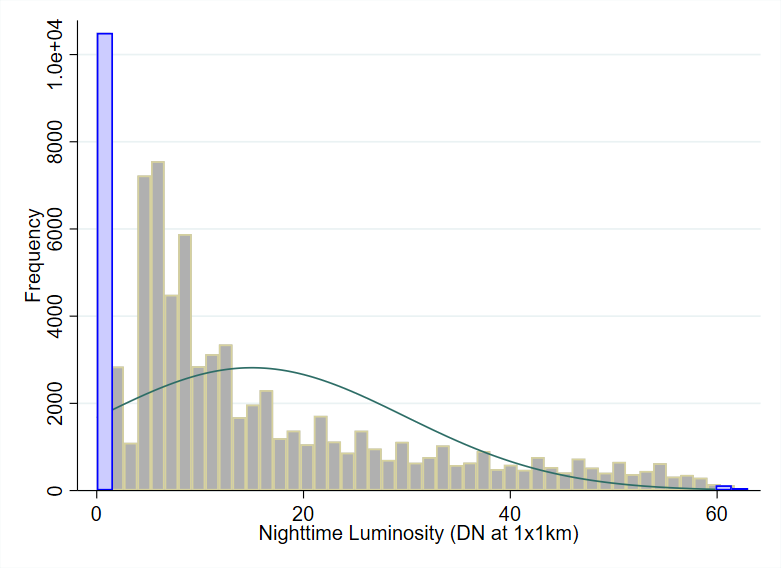
\includegraphics[width=0.5\textwidth]{photos/predata1.png}
        }%
        \subfigure[Log Transformed NTL]{%
           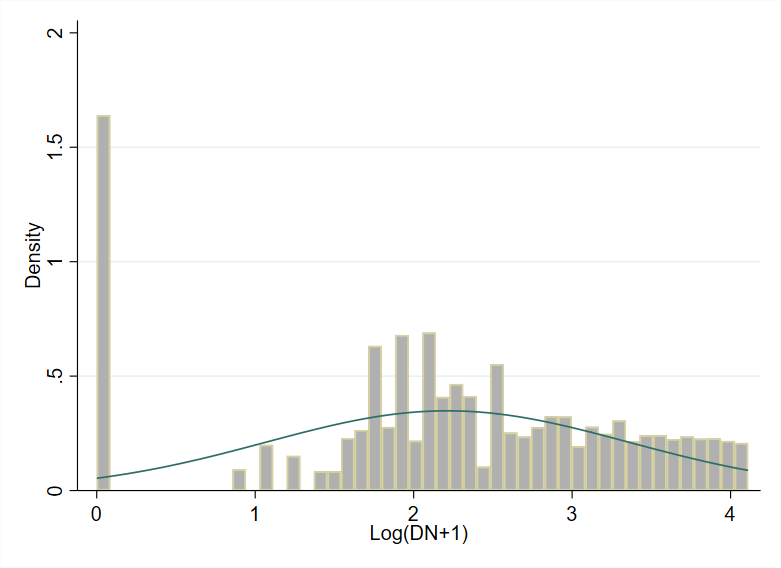
\includegraphics[width=0.5\textwidth]{photos/predata2.png}
        }%
%
    \end{center}
    \caption{%
    Transforming Nighttime Luminosity
     }%
   \floatfoot{ \footnotesize \textit{Source:} Author's elaboration based on DMSP-OLS satellite nighttime lights.}
  
\end{figure}


\par I discuss several strategies to address limitations in my analysis. Let's summarize these strategies:
\begin{itemize}
\item Averaging Data across Satellites: When two satellites were available in a given year, such as in 1994 with the F10 and F12 satellites, I chose to average the data from both satellite sources. This approach helps to reduce measurement errors if they are random in nature.
\item Including Satellite Fixed Effects: If the measurement errors are not random and there are variations in how different satellites capture lights, I account for this potential bias by including satellite-fixed effects in my model. By doing so, I control for within-satellite correlation across years. For example, during 1997-1999, the F12 and F14 satellites were launched; during 2000-2003, it was F14 and F15, and during 2004-2007 it was F15 and F16.
\item Dropping Pixels with High Digital Numbers: To minimize concerns related to top coding or extreme values, I choose to drop all pixels from the sample with digital numbers higher than 60. By excluding these high-value pixels, I aim to mitigate any potential issues associated with outliers in my analysis.
\end{itemize}

\par By employing these strategies, I aim to enhance the accuracy and reliability of my analysis while addressing the limitations associated with satellite data availability, potential biases in satellite-specific measurements, and extreme values in the dataset.


\newpage
\begin{table}[H] \hypertarget{Table 2.A.1}{}
\renewcommand\thetable{2.A.1}
\centering \caption{Summary Statistics after Data Cleansing}
\begin{tabular}{l c c c c c}\hline\hline
\multicolumn{1}{c}{\textbf{Variable}} & \textbf{N}
 & \textbf{Mean}& \textbf{Std. Dev.} &  \textbf{Min.} & \textbf{Max.}\\ \hline
Nighttime Luminosity      & 74,729 & 14.33537 & 14.42692 & 0         & 60       \\
Log(NTL)             & 74,729 & 2.212735 & 1.145026 & 0         & 4.110874 \\
Distance to Historical Center                 & 74,729 & 7.563277 & 4.337439 & .1507614  & 22.15463 \\
Satellite F10                  & 74,729 & .1365333 & .3433563 & 0         & 1        \\
Satellite F12                  & 74,729 & .2730667 & .4455378 & 0         & 1        \\
Satellite F14                  & 74,729 & .3187384 & .4659905 & 0         & 1        \\
Satellite F15                  & 74,729 & .3643298 & .4812449 & 0         & 1        \\
Satellite F16                  & 74,729 & .2733878 & .4457012 & 0         & 1        \\
Satellite F18                  & 74,729 & .1805056 & .3846106 & 0         & 1        \\
Years                 & 74,729 & 2002.489 & 6.339127 & 1992      & 2013     \\
Schengen Entry              & 74,729 & .2716348 & .4448056 & 0         & 1        \\
Longitude of Pixels                    & 74,729 & 15.80379 & 2.709864 & 13.55833  & 26.11667 \\
Latitude of Pixels                    & 74,729 & 50.24682 & 2.824156 & 45.84167  & 57.81667 \\
Longitude of HC               & 74,729 & 15.76925 & 2.732708 & 13.6269   & 26.0376  \\
Latitude of HC              & 74,729 & 50.24786 & 2.83374  & 45.9413   & 57.7773  \\
Pixel ID                   & 74,729 &  -& - & 1         &   3405    \\
Country ID  & 74,729 & - & - & 1         & 10       \\
City ID   & 74,729 & - & -  & 1         & 22       \\ 
Historical Center ID              & 74,729 &  - &- & 1         &  11  \\
Divided city pairs  ID               & 74,729 &  - &-  & 1         & 11       \\
\hline
\hline
\end{tabular}
\end{table}

\newpage
\subsection{Appendix B: Firm Register Data}
\par \textbf{Registers:} I have gathered data on economic entities, including their establishment dates, sectors, and locations, for various cities in different countries. Here is a summary of the data sources I used for each city:
\begin{itemize}
\item  German Cities (Frankfurt (Oder), Görlitz, Gubin): The data for these cities is obtained from the Common Register Portal of the German Federal States.
\item  Polish Cities (Cieszyn, Słubice, Zhořelec, Guben): The data for these cities is collected from the national official business registers in Poland. An alternative data source is the Central Register and Information on Business Activity.
\item  Slovak City (Komárno): The data for this city is obtained from the National Statistical Office of Slovakia.
\item  Hungarian City (Komarom): For this city, I initially obtained the names of registered economic entities from the Hungarian Central Statistical Office (HCSO). Then, using the names, I searched and collected information on the establishment years of these entities from the Ministry of Justice's Company Information and Electronic Business Procedure Service.
\item  Estonian City (Valga): The data for this city is sourced from the Center of Registers and Information Systems in Estonia.
\item  Latvian City (Valka): The data for this city is obtained from the register of enterprises of the Latvian Republic.
\item  Slovenian City (Nova Gorica): The data for this city is sourced from the Agency of the Republic of Slovenia for Public Legal Record.
\item  Italian City (Gorizia): For this city, I used the Italian Digital Database of Companies (AIDA) to gather the required information.
\end{itemize}

Once I have collected the data from these various sources, I merge the datasets to create a comprehensive dataset covering 54,669 economic entities in the divided cities. 




\begin{table}[H] \hypertarget{Table 2.B.1}{}
\renewcommand\thetable{2.B.1}
\centering 
\footnotesize
\caption{Registered Economic Entities in Cities - Availability}
\begin{tabular}{|ll|lll|l|}
\hline
\textbf{City}  & \textbf{Country} & \textbf{Entry Date} & \textbf{NACE} & \textbf{Lat-Long}  & \textbf{N} \\
\hline
\hline
Cieszyn        & Poland           & Y                       & Y        & Y   & 6710     \\

Cesky Tesin    & Czechia          & Y                      & Y        & Y   &4387     \\
\hline
Komarom        & Hungary          & Y                      & Y        & Y      & 998  \\

Komarno        & Slovakia         & Y                       & Y        & Y   & 19354     \\
\hline
Nova Gorica    & Slovenia         & Y                     & Y        & Y    &  7903    \\

Goriza         & Italy            & Y            & Y            & Y          &  1002     \\
\hline
Valga          & Estonia          & Y            & Y           & Y            &650   \\

Valka          & Latvia           & Y            & N            & Y            & 540    \\
\hline
Slubice        & Poland           & Y            & Y           & Y             & 5554 \\

Frankfurt      & Germany          & Y            & N            & Y           & 2035    \\
\hline
Gubin          & Poland           & Y            & Y           & Y          & 458    \\

Guben          & Germany          & Y             & N            & Y           & 640     \\
\hline
Zhorlec        & Poland           & Y            & Y           & Y         &2695      \\

Gorlitz        & Germany          & Y             & N            & Y            & 1743     \\
\hline
Ceske Velenice & Czechia          & Y            & Y           & Y     & 738    \\

Gmund          & Austria          & N             & N            & N         & -    
 \\
\hline
\hline
Total          &           &                         &          &   & 54,669   \\
\hline
\end{tabular}
\end{table}

\subsection {Appendix C: Supplementary}

\begin{figure}[H] \hypertarget{Figure 2.C.1}{}
\renewcommand\thefigure{2.C.1}
\centering
\subfigure[Border Crossing in 1925]{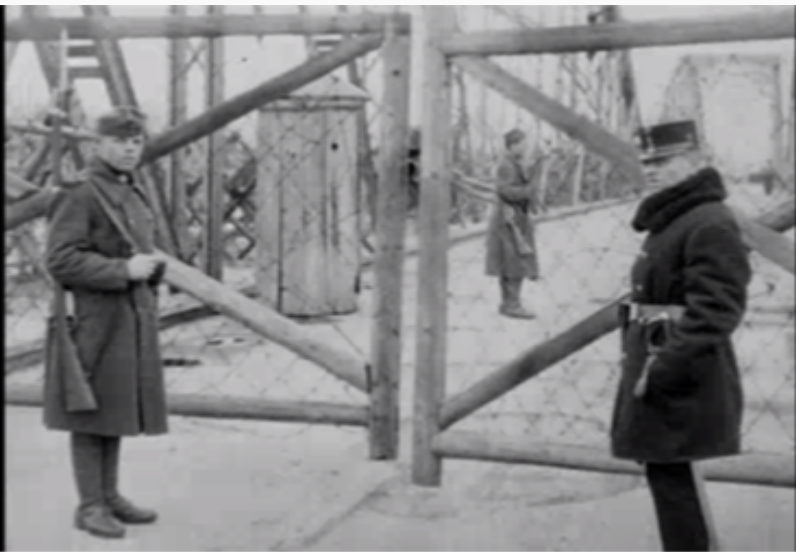
\includegraphics[width=.6\linewidth]{photos/border1925.png}}\hfill
\subfigure[Border Crossing in 2006]{\label{}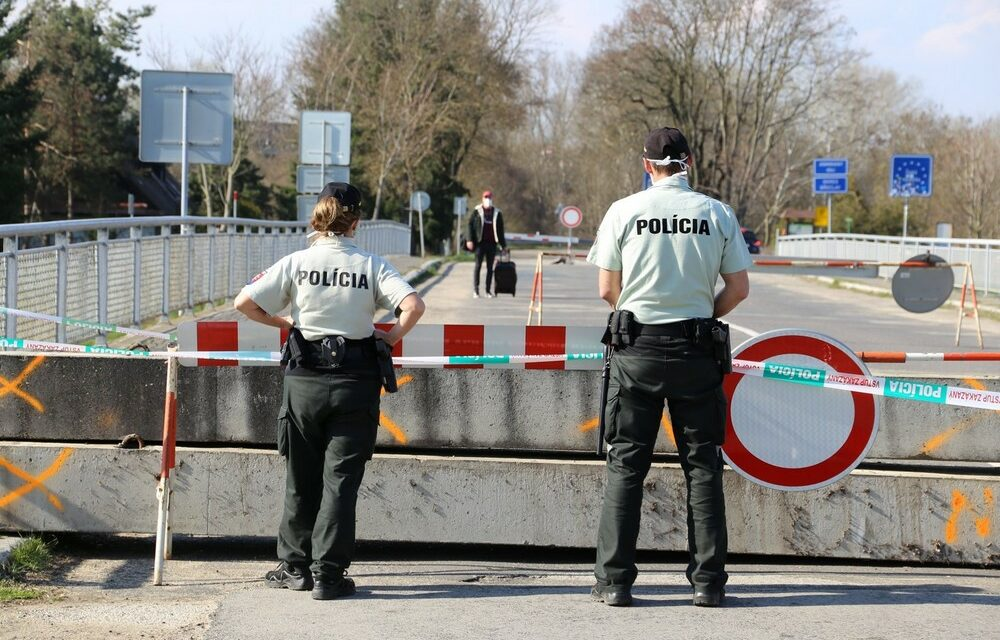
\includegraphics[width=.6\linewidth]{photos/border2006.jpg}}\par 
\caption{Border Crossing between Komarom \& Komarno: in 20th vs. 21st centuries }
{
 \floatfoot{ 
\scriptsize 
\textit{Source:} Photo (a) is taken from a Hungarian silent film from 1925, “The Trianon frontier on the Komárom Bridge” (1925) (available on the following \href{https://filmhiradokonline.hu/watch.php?id=8188}{link}). Photo (a) shows border guards policing the bridge linking Komárom in Hungary with Komárno in Czechoslovakia (today in Slovakia). People pass between the two countries through gates. Photo (b) displays the same area in 2006 where police(wo)man controls on passport checks and border crossing before Schengen came into force in 2008.}}
\end{figure}


\begin{table}[H] \hypertarget{Table 2.C.1}{}
\renewcommand\thetable{2.C.1}
\begin{tabular}{llllll}
\caption{Language and Cultural Differences between Border Cities }
\textbf{Cities}          & \textbf{Language difference \%} & \textbf{Cultural difference \%} & D(No=1) & Respodents & \\
\hline
\hline
Gorizia              & 0.37                         & 0.14                         & 0                      & 54                   &                          \\
Nova Gorica          & 0.20                         & 0.03                         & 0                      & 105                  &                          \\
\hline
Cesky Tesin & 0.04                         & 0.001                        & 1                      & 46                   &                          \\
Ciezsyn    & 0.08                         & 0.03                         & 1                      & 114                  &                          \\
\hline
Frankfurt (Oder)     & 0.33                         & 0.11                         & 0                      & 27                   &                          \\
Slubice              & 0.35                         & 0.11                         & 0                      & 114                  &                          \\
\hline
Guben                & 0.41                         & 0.40                         & 0                      & 54                   &                          \\
Gubin                & 0.34                         & 0.08                         & 0                      & 342                  &                          \\
\hline
Gorlitz              & 0.44                         & 0.10                         & 0                      & 165                  &                          \\
Zgorlec              & 0.26                         & 0.09                         & 0                      & 192                  &                          \\
\hline
Valga                & 0.24                         & 0.23                         & 0                      & 301                  &                          \\
Valka                & 0.33                         & 0.05                         & 0                      & 83                   &                          \\
\hline
Komarom    & 0.02                         & 0.03                         & 1                      & 15                   &                          \\
Komarno   & 0.04                         & 0.06                         & 1                      & 64                   &                          \\
\hline
Gmund                & 0.32                         & 0.001                        & 0                      & 37                   &                          \\
Ceske Velenice       & 0.31                         & 0.09                         & 0                      & 208                  &                          \\
\hline
\hline 
N                    &                              &                              &                        & 1921                 &                        
\\
\end{tabular}
\end{table}
\vspace{0.3cm}
\footnotesize {\textit{Notes:} Auhtor’s calculations based on Interreg A survey, 2022. Column 1 represents divided cities; Columns 2 \& 3 show the shares of respondents who think that language and cultural differences with the neighboring country are very problematic. Column 4 displays the dummy variable constructed based on how many people responded that differences matter - a dummy equals one in cities where a majority of residents do not see these differences as a major problem, and zero otherwise. Column 5 represents the number of respondents in NUTS3 regions where divided cities are located.}

\newpage
\setcounter{secnumdepth}{0} 
\bibliographystyle{apalike}
\bibliography{reference}



\end{document}
